\documentclass[titlepage]{article}
% \usepackage[showframe,pass]{geometry} % show bounding boxes
\usepackage{appendix}
\usepackage{graphicx} % for embedding pictures
\graphicspath{ {screenshots/} }
\usepackage{wrapfig} % for use with figures
\usepackage{tikz} % for doing flow charts and stuff directly inside of latex
\usepackage{framed} % if you want a frame around a figure
\usepackage[hidelinks]{hyperref} % allows embedding links
\usepackage{url} % allows for citing websites and having the URL appear after
\usepackage[T1]{fontenc} % fixes weird font size/encoding issues
\usepackage[utf8]{inputenc} % ensures input is UTF-8
\usepackage{listings} % used to format code
\usepackage{algorithm} % used with the below package to format psuedo code
\usepackage[noend]{algpseudocode} % specifies no end of block messages such as end for.
\usepackage[superscript]{cite} % makes citations superscript
\usepackage{mathtools} % used for all the mathematical notation
\usepackage{etaremune} % enumerate backwards for OSI model
\usepackage{booktabs} % used for tables and making them look slick as
\usepackage{placeins} % used to ensure everything stays inside where it is in the document
\usepackage[nopostdot]{glossaries} % guess what. It manages glossaries
\setacronymstyle{long-short}
\makenoidxglossaries{}

% load the glossary
\loadglsentries{glossary}

% define some colours for code
\definecolor{dkgreen}{rgb}{0,0.6,0}
\definecolor{gray}{rgb}{0.5,0.5,0.5}
\definecolor{mauve}{rgb}{0.58,0,0.82}

% code formatting options
\lstset{%
  frame=tb,
  showstringspaces=false,
  columns=flexible,
  basicstyle={\small\ttfamily},
  numbers=left,
  numberstyle=\tiny\color{gray},
  keywordstyle=\color{blue},
  commentstyle=\color{dkgreen},
  stringstyle=\color{mauve},
  breaklines=true,
  breakatwhitespace=true
}


% diagramming options
\usetikzlibrary{shapes.geometric, arrows, arrows.meta, positioning}

% flow chart styles
\tikzstyle{startstop} = [
  rectangle,
  rounded corners,
  minimum width=3cm,
  minimum height=1cm,
  text centered,
  draw=black,
  inner sep=0,
  fill=red!30
]
\tikzstyle{io} = [
  trapezium,
  trapezium left angle=60,
  trapezium right angle=120,
  minimum width=3cm,
  minimum height=1cm,
  text centered,
  text width=3cm,
  inner sep=0,
  draw=black,
  trapezium stretches=true,
  fill=blue!30
]
\tikzstyle{process} = [
  rectangle,
  minimum width=3cm,
  minimum height=1cm,
  text centered,
  text width=3cm,
  inner sep=0,
  draw=black,
  fill=orange!30
]
\tikzstyle{decision} = [
  diamond,
  minimum width=3cm,
  minimum height=1cm,
  text centered,
  draw=black,
  aspect=2,
  inner sep=0,
  fill=green!30
]
\tikzstyle{arrow} = [
  thick,
  ->,
  =stealth
]

% data flow diagram styles
\tikzstyle{function} = [
  circle,
  inner sep=0pt,
  draw=black,
  minimum width=1cm,
  minimum height=1cm,
  text width=2cm,
  text centered,
  fill=red!20
]
\tikzstyle{inputoutput} = [
  rectangle,
  draw=black,
  minimum width=3cm,
  minimum height=1cm,
  text width=3cm,
  text centered,
  fill=blue!20
]
\tikzstyle{datastore} = [
  rectangle,
  inner sep=0pt,
  minimum height=1cm,
  minimum width=3cm,
  text width=3cm,
  text centered,
  fill=green!20
]
\tikzstyle{method} = [
  rectangle,
  draw=black,
  fill=gray!30,
  minimum width=2cm,
  minimum height=0.5cm,
  text centered
]

% ladder diagram lines
\tikzstyle{connecting arrow} = [-{Latex[length=2mm, width=3mm, green]}]
\tikzstyle{closing arrow} = [-{Latex[length=2mm, width=3mm, red]}]
\tikzstyle{normal arrow} = [-{Latex[length=2mm, width=3mm, blue]}]
\tikzstyle{with slope} = [above, midway, sloped]


% forces [sub]sections to contain everything that is defined before the next one
\let\Oldsection\section{}
\renewcommand{\section}{\clearpage\FloatBarrier\Oldsection}

\let\Oldsubsection\subsection{}
\renewcommand{\subsection}{\FloatBarrier\Oldsubsection}

\let\Oldsubsubsection\subsubsection{}
\renewcommand{\subsubsection}{\FloatBarrier\Oldsubsubsection}


% title
\author{Sam Leonard}
\title{A Level Computer Science Non-Examined Assessment (NEA)}
\date{} % this forces no date to be shown


% paragraph styling
\setlength{\parindent}{0cm}

\begin{document}

\maketitle

\tableofcontents

\setlength{\parskip}{6pt plus 1pt minus 1pt}

\section{Analysis}

\subsection{Identification and Background to the Problem}

The problem my project tries to solve is how to look at devices on a network from a 
``\gls{bbox}'' perspective and gain information about what \glspl{service} are running.
Services are programs whose entire purpose is to provide a \textit{\gls{service}} to other programs.
For example a server hosting a website would be running a \gls{service} whose purpose is to send the 
webpage to people who try to connect to the website.

There are a number of steps a device has to go through from when it is turned on until it
can connect to the internet.
There are many more steps than those listed below, but the most important ones are.

\begin{enumerate}
  \item{Loading networking \glspl{driver}}
  \item{Starting \gls{dhcp} \gls{daemon}}
  \item{Broadcasting \gls{dhcp} request for an \gls{ipaddr}}
  \item{Obtaining assigned an \gls{ipaddr}}
\end{enumerate}

Starting from a Linux computer being switched on, the first step is that the \gls{kernel} needs to load the 
networking \glspl{driver}. The \gls{kernel} is the basis for the operating system, it is what 
interacts with the hardware in the most fundamental way. Drivers are small bits of code which 
the \gls{kernel} can load in order to interact with certain hardware modules.
These can range from graphics drivers for games to use graphics cards, to networking drivers
which interact with the \gls{nic}.

Once the \gls{kernel} has loaded the required \glspl{driver} and the system has booted, the 
networking `\glspl{daemon}' must be started. In Linux, a \gls{daemon} is a program that runs all the 
time in the background to serve a specific purpose or utility. For example, when I start my laptop,
the following \glspl{daemon} start: \gls{upow} (power management), \gls{sysd} (manages the creation 
of all processes), \gls{dbus} (manages inter-process communication), iwd (manages my WiFi 
connections) and finally \gls{dhcpcd}, which manages all interactions with the network around 
\gls{dhcp}.

Once the \glspl{daemon} are all started, the \gls{dhcp} client can issue commands to the 
daemon for it to carry out. The \gls{dhcp} client is simply a daemon that runs in the background to 
carry out any interactions between the current machine and the \gls{dhcp} server. The \gls{dhcp} 
server is normally the WiFi router or network switch for the local network and it manages a list of 
which computer has which \gls{ipaddr} and negotiates with new computers trying to join a network to 
get them a free \gls{ipaddr}. The \gls{dhcp} client starts the \gls{dhcp} address negotiation with 
the server by sending a discover message with the address 255.255.255.255, which is the IP limited 
broadcast address, which means that whatever is listening at the other end will forward this 
\gls{pkt} on to everyone on the \gls{subnet}. When the \gls{dhcp} \gls{server} (normally the router, 
sometimes a separate machine) on the subnet receives this message it reserves a free \gls{ipaddr} 
for that client and then responds with a \gls{dhcp} offer that contains the address the 
\gls{server} is offering, the length of time the address is valid for and the \gls{subnet} mask of 
the network. The client must then respond with a \gls{dhcp} request message to request the offered 
address, this is in case of multiple DHCP servers offering addresses. Finally the \gls{dhcp} server 
responds with a \gls{dhcp} acknowledge message showing that it has received the request
(see Figure~\ref{dhcpdiagram}).

\begin{figure}[H]

  \begin{framed}

  \centering
  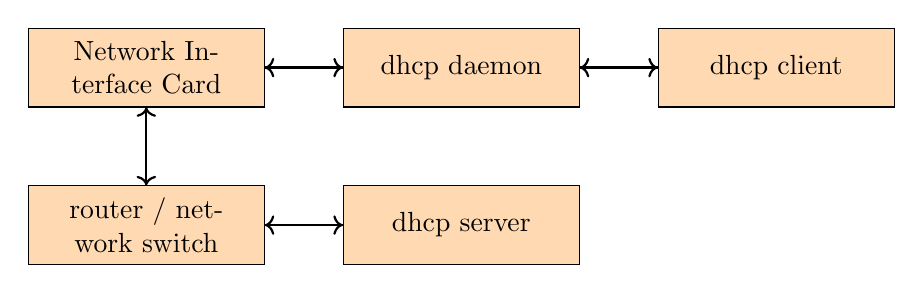
\begin{tikzpicture}[node distance=2cm]

    \node (nic) [process] {Network Interface Card};
    \node (router) [process, below of=nic] {router / network switch};
    \node (daemon) [process, right of=nic, xshift=2cm] {\gls{dhcp} daemon};
    \node (client) [process, right of=daemon, xshift=2cm] {\gls{dhcp} client};
    \node (server) [process, right of=router, xshift=2cm] {\gls{dhcp} server};

    \draw [arrow] (nic) -- (router);
    \draw [arrow] (router) -- (nic);
    \draw [arrow] (server) -- (router);
    \draw [arrow] (router) -- (server);
    \draw [arrow] (nic) -- (daemon);
    \draw [arrow] (daemon) -- (nic);
    \draw [arrow] (client) -- (daemon);
    \draw [arrow] (daemon) -- (client);

  \end{tikzpicture}

  \end{framed}

  \caption{\textit{%
    A block diagram showing the relationship between
    different elements of a \gls{dhcp} negotiation.
  }}\label{dhcpdiagram}
\end{figure}

Figure~\ref{dhcp_negotiate} shows a \gls{pkt} capture from my laptop where I turned WiFi off, 
started Wireshark listening and plugged in an Ethernet cable. 
Wireshark is a program which intercepts all the network communications
on a single computer and records them to a file\cite{download:wireshark}.
It also displays them to the user, and is capable of performing an analysis and
dissection of each the protocols used.
This means that I can record the \gls{dhcp} negotiation shown below and 
show it to you using Wireshark to get all the information out of the packets
being sent over the wire.
For a definition of \glspl{pkt} see Page~\pageref{packetdef}.

For the sake of clarity, the Figure displays Wireshark showing only the \gls{dhcp} \glspl{pkt},
so that the \gls{dhcp} negotiation can be clearly seen, including the \\
255.255.255.255 limited broadcast destination address
and the 0.0.0.0 unassigned address in the source column.

\begin{figure}[H]
  \centering
  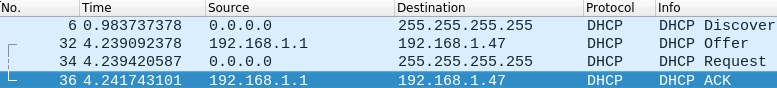
\includegraphics[width=\textwidth]{dhcp_negotiation.png}
  \caption{\textit{\gls{dhcp} address negotiation.}}\label{dhcp_negotiate}
\end{figure}

All computer networking is encapsulated in the \gls{osi} which has 7 layers:

\begin{etaremune}
  \item{Application: \gls{api}s, etc\ldots}
  \item{Presentation: encryption/decryption, encoding/decoding, decompression etc\ldots}
  \item{Session: Managing sessions, \gls{php} session IDs etc\ldots}
  \item{Transport: TCP and UDP among others.}
  \item{Network: ICMP and IP among others.}
  \item{Data Link: MAC addressing, Ethernet protocol etc\ldots}
  \item{Physical: The physical Ethernet cabling/\gls{nic}.}
\end{etaremune}

\begin{figure}[H]
  \centering
  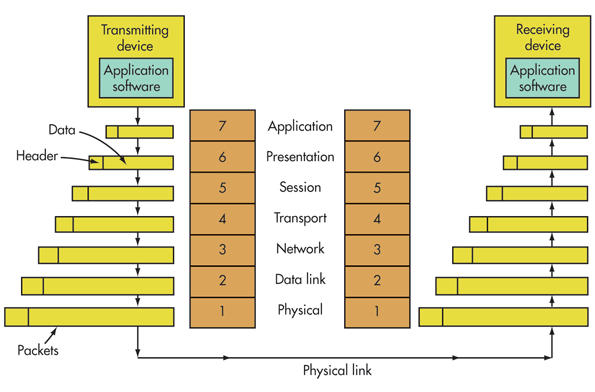
\includegraphics[width=\textwidth]{osi_model.png}
    \caption{\textit{%
    \gls{osi} diagram, source: https://www.electronicdesign.com.
}}\label{osi_model}
\end{figure}
Each of these layers is essential to the running of the internet but a single communication might 
not include all of the layers. These communications are all based on the most fundamental part of 
the internet: the \gls{pkt}. 

Packets\label{packetdef} are sequences of ones and zeros sent between computers which 
are used to transfer data as well as to control how networks function. They consist of different 
layers of information; the innermost layer contains the data being transferred, and the other
layers specify where the packet should go next.
When \glspl{pkt} are sent between computers, a certain number of layers are stripped off by,
each computer so that it knows where to send the \gls{pkt} next, at which point it will add
all the layers back again, this time with the instructions needed to go from the current computer
to the next one on its route. Each of these layers actually consists of a number of fields at the
start, called a \gls{header}; some layers also append a footer to the end of the packet.
The actual data being transferred in the packet can be anything.
As an example, \gls{http} transfers websites using \gls{html} files and images. In particular,
there are two pieces of information stored in headers which together define the final destination
of the packet: the \gls{ipaddr} and the \gls{port} number.
The \gls{ipaddr} defines the destination machine and the \gls{port} number
defines which ``port'' on the remote machine the packet should be sent to. Ports are essential
entrances to a computer; for example, if a computer were a hotel, the \gls{ipaddr} would be the
address of the hotel, and the \gls{port} number would be the room inside the hotel.
There are 65535 \glspl{port} and 0 is a special reserved port.
There are this many ports because the port field in \gls{tcp} and \gls{udp} is 16 bits long and the maximum
value for a 16 bit unsigned integer in 65535.
Both \gls{tcp} and \gls{udp} use \glspl{port}; \gls{tcp} \glspl{port} are mainly used for
transferring data where reliability is a concern, as \gls{tcp} has built in checks for packet loss
whereas \gls{udp} does not.
For this reason, \gls{udp} is used for purposes where speed is more important
and missing some data is inconsequential, such as video streaming and playing online games. 

I would like to illustrate how ports and packets work using the example of getting a very simple
static HTML page with an image inside.
The code for the page is shown in Listing~\ref{examplepage}.
In Figure~\ref{basicwebpage} you can see how the page renders.
However, far more interesting is how the browser retrieved the page. In Figure~\ref{getrequest}
you can see the full sequence of \glspl{pkt} that were exchanged for the 
browser to get the resources it needed to render the page. The page is hosted using Python3's 
http.server module, which is a quick and easy way to serve HTML pages and other content locally,
without the hassle of setting up a full blown web server such as Nginx or Apache.
Python's http.server makes the current directory open on port 8000.
From there, navigating to /example.html will render the page.
Breaking Figure~\ref{getrequest} down, \gls{pkt} one shows the browser receiving the request from the user to 
display \verb|http://192.168.1.47:8000/example.html| and attempting to connect to 192.168.1.47 on 
port 8000. Packets two and three show the negotiation of this request through to the full connection 
being made. The browser now makes an \gls{http} GET request for the page example.html over the 
established TCP connection, as shown in \gls{pkt} 4. The server then acknowledges the request and 
sends a \gls{pkt} with the PSH flag set, as shown in \glspl{pkt} 6 and 7.
The PSH flag in the \gls{tcp} header is used to notify the client that the server is ready to
push the data (in this case example.html) to the client.
The browser then sends back an acknowledgement and the server sends the page as shown in \glspl{pkt} 7 and 8. 
Finally, the browser sends an acknowledgement of having received the page before initiating a 
graceful session teardown by sending a FIN ACK \gls{pkt}, which indicates the end of a session.
Having received the FIN ACK packet, the server acknowledges this by sending an ACK packet back
to the client, completing the graceful teardown.
This process is repeated when the browser parses the HTML and identifies there is an image which it needs to 
get from the server as well. Because the image is a large file, it takes more \glspl{pkt} to
transfer the required data.
In Figure~\ref{ladder} you can see a ladder diagram which shows the entire transaction symbolically.
I have also colour coded Figure~\ref{ladder} with green arrow heads to the initial handshakes,
blue for the HTTP protocol transactions and red for the TCP connection teardown packets.

The \gls{osi} described in Figure~\ref{osi_model} can be seen in action in Figures~\ref{basicwebpage},~\ref{getrequest} and~\ref{deconstructed}.
Figure~\ref{basicwebpage} shows levels 6 and 7 of the \gls{osi}.
Levels 4 and 5 can be seen in figure~\ref{getrequest} in the form of the \gls{tcp}
session negotiation and transferring the picture and example.html.
Level 3/2/1 are shown in Figure~\ref{deconstructed} where you can see the IP layer information
along with Ethernet II and finally frame 4 which is the bytes that went down the wire.

\begin{figure}[H]
  \centering
  \begin{framed}
  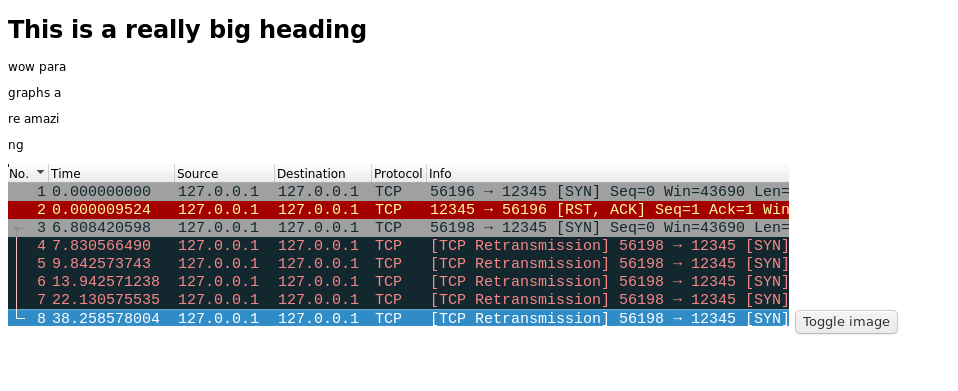
\includegraphics[width=\textwidth]{basic_webpage.png}
  \end{framed}
    \caption{\textit{%
    A basic static \gls{html} webpage.
}}\label{basicwebpage}
\end{figure}

\begin{figure}[H]
  \centering
  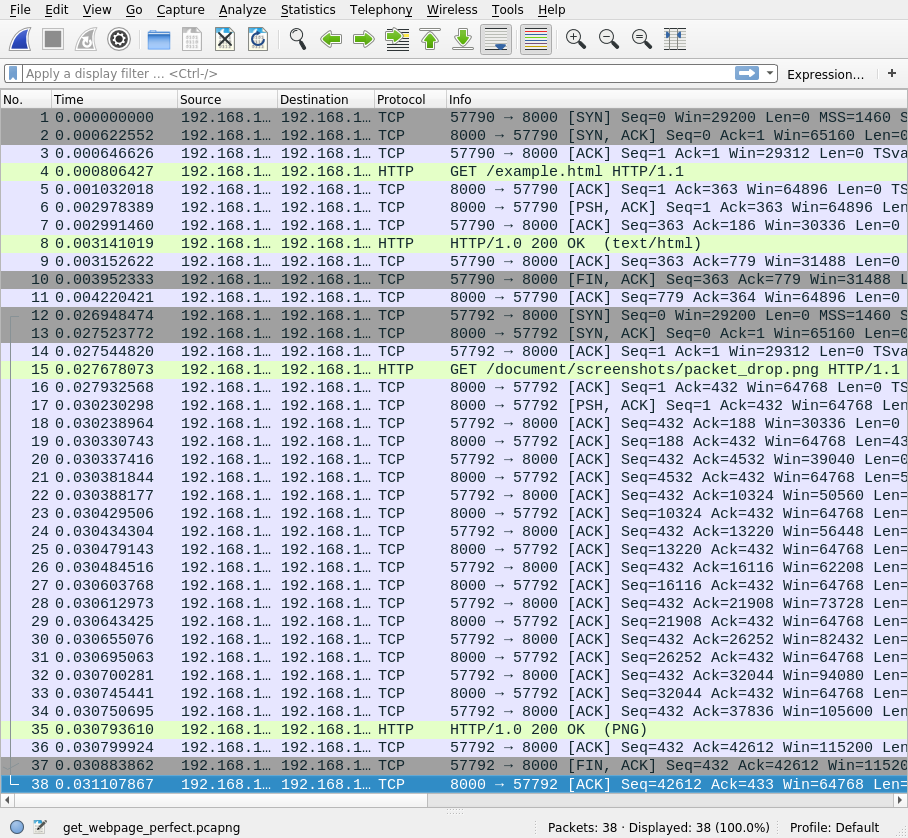
\includegraphics[width=\textwidth]{website_get.png}
    \caption{\textit{%
    A full chain of \glspl{pkt} that shows retrieving a basic webpage
    from the server.
}}\label{getrequest}
\end{figure}

\begin{figure}[H]
  \centering
  \begin{framed}
  
\begin{tikzpicture}
    \node[rectangle,minimum width=.8\textwidth,minimum height=.8\textheight] (ladder) {};
      \draw[black,very thick] (ladder.north west) -- (ladder.south west);
      \draw[black,very thick] (ladder.north east) -- (ladder.south east);
    \node[above of=ladder, xshift=-4.5cm,yshift=7cm] (local 0) {local machine};
    \node[above of=ladder, xshift=4.5cm, yshift=7cm] (web 0) {webserver};
    \foreach \i [count=\j from 0]in {1,...,14}{
      \node [below=0.85cm of local \j] (local \i) {};
      \node [below=0.85cm of web \j] (web \i) {};
    }

    \draw[connecting arrow] (local 0) -- node[with slope] {SYN} (web 1);
    \draw[connecting arrow]   (web 1) -- node[with slope] {SYN ACK} (local 2);
    \draw[connecting arrow] (local 2) -- node[with slope] {ACK} (web 3);
    \draw[normal arrow]     (local 3) -- node[with slope] {HTTP GET /example.html} (web 4);
    \draw[normal arrow]       (web 4) -- node[with slope] {HTTP 200 OK} (local 5);
    \draw[closing arrow]    (local 5) -- node[with slope] {FIN ACK} (web 6);
    \draw[closing arrow]      (web 6) -- node[with slope] {ACK} (local 7);
    \draw[connecting arrow] (local 7) -- node[with slope] {SYN} (web 8);
    \draw[connecting arrow]   (web 8) -- node[with slope] {SYN ACK} (local 9);
    \draw[connecting arrow] (local 9) -- node[with slope] {ACK} (web 10);
    \draw[normal arrow]    (local 10) -- node[with slope] {HTTP GET /document/screenshots/packet\_drop.png} (web 11);
    \draw[normal arrow]      (web 11) -- node[with slope] {HTTP 200 OK} (local 12);
    \draw[closing arrow]   (local 12) -- node[with slope] {FIN ACK} (web 13);
    \draw[closing arrow]     (web 13) -- node[with slope] {ACK} (local 14);

  \end{tikzpicture}
  \end{framed}
    \caption{\textit{%
    A ladder diagram showing the transaction in Figure~\ref{getrequest}.
}}\label{ladder}
\end{figure}

\begin{figure}[H]
  \centering
  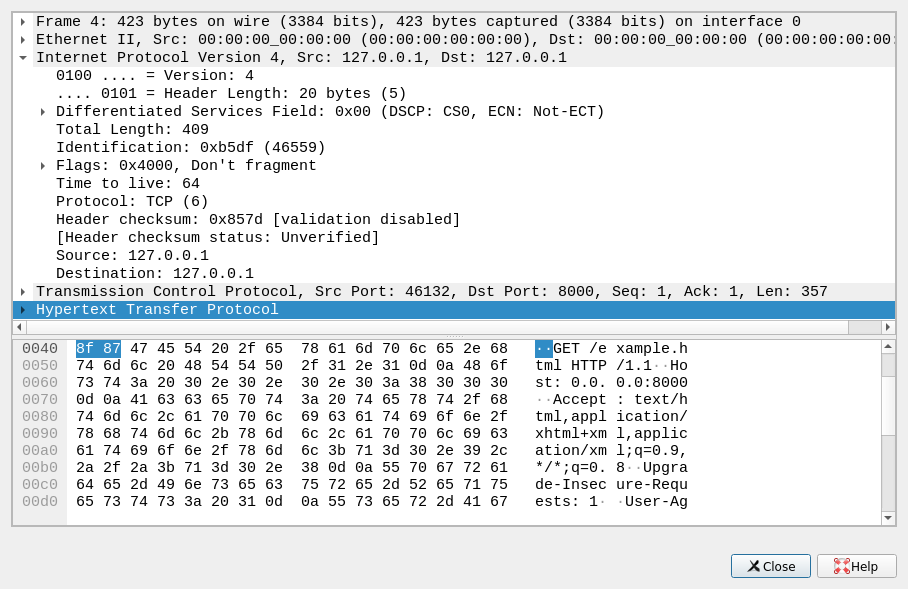
\includegraphics[width=\textwidth]{deconstructed_packet.png}
  \caption{\textit{%
    A look inside a TCP \gls{pkt}.
}}\label{deconstructed}
\end{figure}

\lstset{language=HTML}
  \lstinputlisting[caption={\textit{\textit{example.html}}}, label={examplepage}]{../example.html}

\subsection{Analysis of problem}

To reiterate, the problem my project tries to solve is how to look at devices on a network from a 
``\gls{bbox}'' perspective and gain information about what \glspl{service} are running.
The difficulty with looking at a network from the outside is that the purpose of the network is to 
allow communication within the network, thus very little is exposed externally. This presents a 
challenge, as we want to know not only what machines are on the network, but also what
services are running on each machine.
This is not always possible, owing to the limited information that \glspl{service} reveal about 
themselves. Firewalls also play a large part in making network scanning difficult, as sometimes they 
simply drop \glspl{pkt} instead of sending a \gls{tcp} RST \gls{pkt} (reset connection \gls{pkt}). 
Dropping a packet means that when a packet is received, no response is sent back \textendash{}
as if the connection was just ``dropped''.
When firewalls drop \glspl{pkt}, it becomes exponentially more difficult to determine the
state of any port on the target machine, as you don't know whether 
your \gls{pkt} was corrupted, or lost in transit, or if it was just dropped.
 \\\\ To demonstrate this 
I will show three things:

\begin{enumerate}
  \item{A successful connection over \gls{tcp}.}
  \item{An attempted connection to a closed port.}
  \item{An attempted connection with a firewall rule to drop packets.}
\end{enumerate}

\subsubsection{Successful connection over TCP}
For a \gls{tcp} connection to be established there is a 
three-way handshake between the communicating machines.
Initially, the machine trying to establish the connection sends a \gls{tcp} SYN packet to the other machine.
This packet holds a dual purpose\cite{rfc:tcp}: to ask for a connection, and, if it is accepted, to SYNchronise the 
sequence numbers being used to detect whether packets have been lost in transport.
The receiving machine then replies with a \gls{tcp} SYN ACK, which confirms the starting sequence
number with SYN, and ACKnowledges the connection request.
The sending machine then acknowledges this by sending a final \gls{tcp} ACK packet back. 
This connection initialisation is shown in Figure~\ref{data_transfer} by packets one, two and three. 
Data transfer can then commence by sending a \gls{tcp} packet with the PSH and ACK flags set, along 
with the data in the data portion of the packet. This is shown in Figure~\ref{data}, where Wireshark
allows us to take a look inside the packet to see the data being sent, along with the 
PSH and ACK flags being set. 

The code I used to generate these packet captures is shown in
Figures~\ref{sender} and~\ref{receiver}.
Breaking the code down, Figure~\ref{receiver} shows me initialising a 
socket object\cite{python:socket}, then I bind it to localhost (127.0.0.1) port 12345.
Localhost is just an address which allows connections between programs running on the
same computer to be looped back onto the current machine, hence its alternative name:
the loopback address. 
The next line of code instructs the machine to listen for incoming connections.
The program accepts the connection in Figure~\ref{sender}, line 3.
I then tell the program to listen for up to 1024 bytes in the data part of any TCP packets sent.
The program in Figure~\ref{sender} then sends some data which we then see
printed to the screen in Figure~\ref{receiver}, both programs 
then close the connection.

\begin{figure}[H]
  \centering
  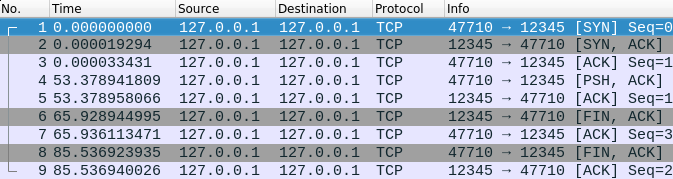
\includegraphics[width=\textwidth]{data_transfer.png}
  \caption{\textit{%
    Packets starting a TCP session, transferring some data then ending it.
}}\label{data_transfer}
\end{figure}

\begin{figure}[H]
  \centering
  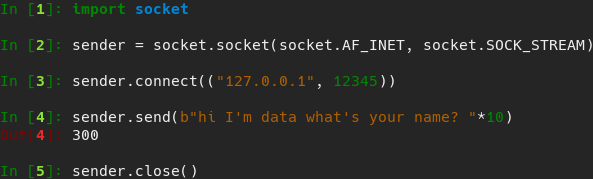
\includegraphics[width=\textwidth]{sender.png}
  \caption{\textit{%
    Transferring some basic text data over a TCP connection.
}}\label{sender}
\end{figure}

\begin{figure}[H]
  \centering
  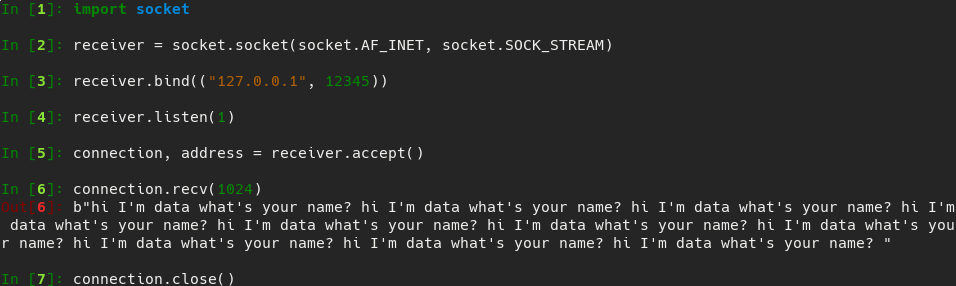
\includegraphics[width=\textwidth]{receiver.png}
  \caption{\textit{%
    Receiving some basic text data over a TCP connection.
}}\label{receiver}
\end{figure}

\begin{figure}[H]
  \centering
  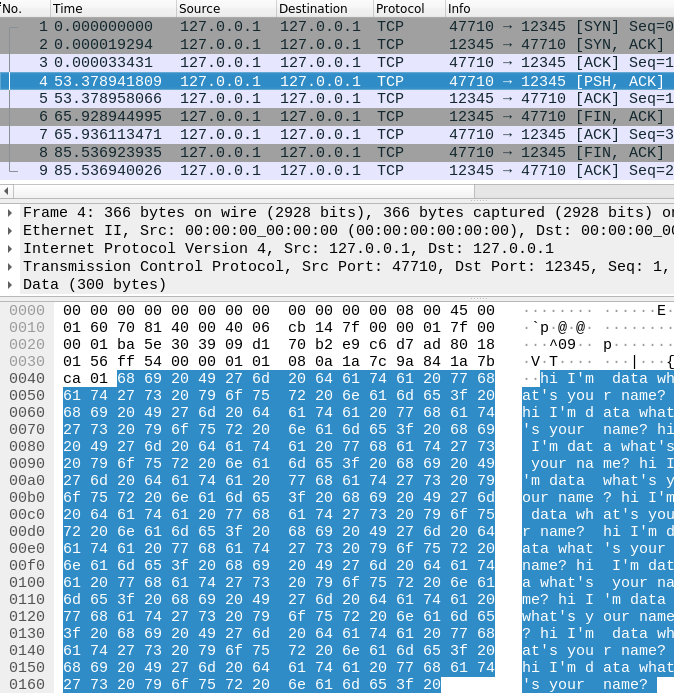
\includegraphics[width=\textwidth]{data.png}
  \caption{\textit{%
    Highlighted packet carrying the data being transferred in Figure~\ref{sender}.
}}\label{data}
\end{figure}

\subsubsection{An attempted connection to a closed port}
In Figure~\ref{firewall} shows my program beginning by sending the same \gls{tcp} SYN
packet as we saw in the attempted connection to an open port discussed above.
The difference comes in the next packet with the \gls{tcp} RST flag being sent
back. This flag resets the connection\cite{rfc:tcp}, or if the connection is not yet established,
as in this case, it means that the port is closed, hence why the packet is highlighted red
in Figure~\ref{firewall}. The code used to generate this is shown in Figure~\ref{firewall_code};
line two shows the initialisation of a socket object. In line 3 the program tries to connect
to port 12345 on localhost again, except this time we get a connection refused error back.
This shows us that the remote host sent a \gls{tcp} RST packet back, which is reflected in
Figure~\ref{firewall}.

\begin{figure}[H]
  \centering
  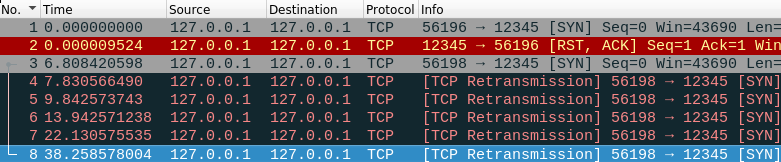
\includegraphics[width=\textwidth]{packet_drop.png}
  \caption{\textit{%
    Attempted connection to a closed port with and without firewall rule to drop \glspl{pkt}.
}}\label{firewall}
\end{figure}

\begin{figure}[H]
  \centering
  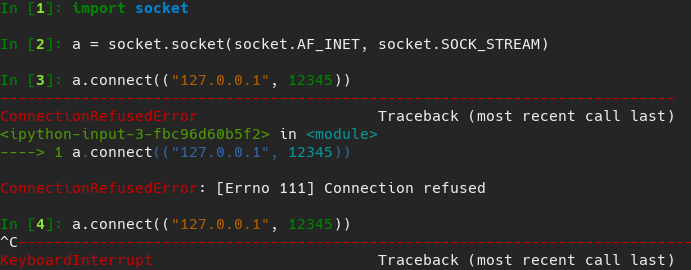
\includegraphics[width=\textwidth]{packet_drop_code.png}
  \caption{\textit{%
    The code used to produce firewall \gls{pkt} dropping example in Figure~\ref{firewall}.
}}\label{firewall_code}
\end{figure}

\subsubsection{An attempted connection with a firewall rule to drop packets}
I would like to commence this section by explaining a bit about firewalls and how they work.
Firewalls are essentially the gatekeepers of the internet;
they decide whether or not a packet is passed on.
Firewalls work by a set of rules which decide what to do with a particular packet.
Such a rule might be that it is coming from a certain \gls{ipaddr} or has a particular destination port.
The actions taken after the packet has had its fate decided by the rules can be one
of the following three (on iptables on Linux):
ACCEPT, DROP and RETURN.\@
ACCEPT does exactly what you think it would and lets the packet through;
DROP simply drops the packet and sends no reply whatsoever:
RETURN is more complicated and has no effect on how port scanning is done,
and as such we will ignore it. A common set of rules for something like a webserver
would be to DROP all incoming packets and then allow exceptions for 
certain ports i.e.\ port 80 for \gls{http} or 443 for \gls{https}.
For demonstration purposes I will be using a Linux utility called iptables for
implementing all firewall rules on my system.
Packet number three in Figure~\ref{firewall} corresponds to line 4 of the code in Figure~\ref{firewall_code},
the difference being that in Figure~\ref{firewall_code} I have enabled a firewall rule to drop all \glspl{pkt} from the 
address 127.0.0.1, using the iptables command as so: \verb$iptables -I INPUT -s 127.0.0.1 -j DROP$. 
This command directs that all \glspl{pkt} arriving (\verb|-I INPUT|) with source address 127.0.0.1 
(\verb|-s 127.0.0.1|) are dropped, with no response sent (\verb|-j DROP|)\cite{man:iptables}. With this firewall rule in 
place you can see in Figure~\ref{firewall}, \gls{pkt} 3 receives no response, and as such Python 
assumes that the \gls{pkt} just got lost and tries to send the \gls{pkt} again repeatedly.
This continued for more than 30 seconds before I stopped it, as shown by the time column in 
Figure~\ref{firewall}, and the final \verb|KeyboardInterrupt| in Figure~\ref{firewall_code}.
The amount of time that a system will continue trying to reconnect depends on the OS and other 
factors, but the minimum time is 100 seconds, as specified by RFC 1122\cite{rfc:hostrequirements}.
On most systems, the timeout is between 13 and 30 minutes, according to the Linux
manual page on \gls{tcp} reproduced below\cite{man:tcp}.

\begin{verbatim}
man 7 tcp:
tcp_retries2 (integer; default: 15; since Linux 2.2)
  The maximum number of times a TCP packet is retransmitted in
  established state before giving up. The default value is 15,
  which corresponds to a duration of approximately between 13 to
  30 minutes, depending on the retransmission timeout. The RFC
  1122 specified minimum limit of 100 seconds is typically deemed
  too short.
\end{verbatim}

\subsubsection{Project aims and methods}\label{pythonreason}
Having explained firewalls, how they affect port scanning and other things above, I will now explain 
what I am actually trying to achieve with my project and how I am going to do it. I am trying to 
make a tool similar to nmap~\cite{download:nmap}, which will be able to detect the state
of ports on remote machines (as in whether the port is open/closed or filtered etc.);
detect which hosts are up on a subnet; and detect what services are listening behind any of the ports.
I am going to be writing in Python version 3.7.2, as it is the latest stable release of Python 3,
and has many features such as f-strings which are not in even fairly recent versions such as 3.5.
F-strings allow for a clear and consistent string formatting syntax, which I will use extensively.
I have chosen Python in particular, because it is very readable and has extensive low level bindings
to kernel syscalls with the socket module allowing me to write code quickly that is easily 
understandable and has a clear purpose. Python enables me to use low level networking 
functions, and even change the behaviour at this low level with \verb|socket.setsockopt|. As well 
as this, the socket module allows me to open sockets that communicate using many different protocols 
such as \gls{tcp}, \gls{udp} and \gls{icmp}. These features combine to make 
Python a great language for writing networking software with a high level of abstraction. In regards 
to the \gls{osi}, my code will sit with the user interface at level 7 specifying what to do at a high 
level, and the actual scanning takes place at levels 3, 4 and 5, with host detection being at level 
3. Port scanning will be taking place at level 4 for \gls{tcp} SYN scanning and \gls{udp} scanning,
whereas \verb|connect()| scanning and version detection will sit at level 5. Finally, I will look at 
what is actually handling all of the networking on my machine. My machine runs Linux, and as such all 
networking is handled by system calls to the Linux kernel. For example, the \verb|socket.connect| 
method is just a call to the underlying Linux kernel's connect syscall, but presents a kinder call 
signature to the user, as the Python socket library does some processing before the syscall is made.

\subsection{Success Criteria}

\begin{enumerate}

  \item{%
    Probe another computer's networking from a \gls{bbox} perspective.
  }\label{blackbox}
  \item{%
    To help the user with usage/help messages when prompted.  
  }\label{usage}
  \item{%
    Translate \gls{cidr}-specified subnets into a list of domains.
  }\label{cidr}
  \item{%
    Send \gls{icmp} ECHO requests to determine whether a machine is active
    or not.
  }\label{ping}
  \item{%
    Perform any scan type without first checking whether the host is up.
  }\label{nocheck}
  \item{%
    Detect whether a TCP port is open (can be connected to).
  }\label{tcpopen}
  \item{%
    Detect whether a TCP port is closed (will refuse connections).
  }\label{tcpclosed}
  \item{%
    Detect whether a TCP port is filtered (a firewall is
    preventing or monitoring access).
  }\label{tcpfiltered}
  \item{%
    Detect whether a UDP port is open (can be connected to).
  }\label{udpopen}
  \item{%
    Detect whether a UDP port is closed (will refuse connections).
  }\label{udpclosed}
  \item{%
    Detect whether a UDP port is filtered (a firewall is
    preventing or monitoring access).
  }\label{udpfiltered}
  \item{%
    Detect the operating system of another machine on the network
    solely from sending packets to the machine and interpreting the responses.
  }\label{osdetect}
  \item{%
    Detect what service is listening behind a port.
  }\label{servicedetect}
  \item{%
    Detect the version of the service running behind a port.
  }\label{versiondetect}

\end{enumerate}

\subsection{Description of existing solutions}

Nmap is currently the most popular tool for doing \gls{port} scanning and host enumeration.
It supports the scanning types for determining information about remote hosts.

\begin{itemize}
  \item{\gls{tcp}:\ SYN}
  \item{\gls{tcp}:\ \verb|Connect()|}
  \item{\gls{tcp}:\ ACK}
  \item{\gls{tcp}:\ Window}
  \item{\gls{tcp}:\ Maimon}
  \item{\gls{tcp}:\ Null}
  \item{\gls{tcp}:\ FIN}
  \item{\gls{tcp}:\ Xmas}
  \item{\gls{udp}}
  \item{Zombie host/idle}
  \item{\gls{sctp}:\ INIT}
  \item{\gls{sctp}:\ COOKIE-ECHO}
  \item{IP protocol scan}
  \item{\gls{ftp}:\ bounce scan}
\end{itemize}

As well as supporting a vast array of scanning types,
Nmap can also perform \gls{service} and version detection,
and operating system detection via custom probes. It also has script scanning, which allows the 
user to write a script specifying exactly how they want to scan, e.g.\ to circumvent \gls{port 
knocking} (where \glspl{pkt} must be sent to a sequence of \glspl{port} in order before access to 
the final\gls{port}is allowed). It supports a plethora of options to avoid firewalls or 
\gls{ids}, such as sending \glspl{pkt} with spoofed \glspl{csum}/source addresses, and sending decoy 
probes. Nmap can do many more things than I have listed above, and indeed there is an
entire book on using nmap (\href{https://nmap.org/book/}{https://nmap.org/book/}).
Figure~\ref{nmapflow} shows the logical structure behind nmap scanning a network.

\begin{figure}[H]
  \hspace{2cm}
  \begin{framed}

  \centering
  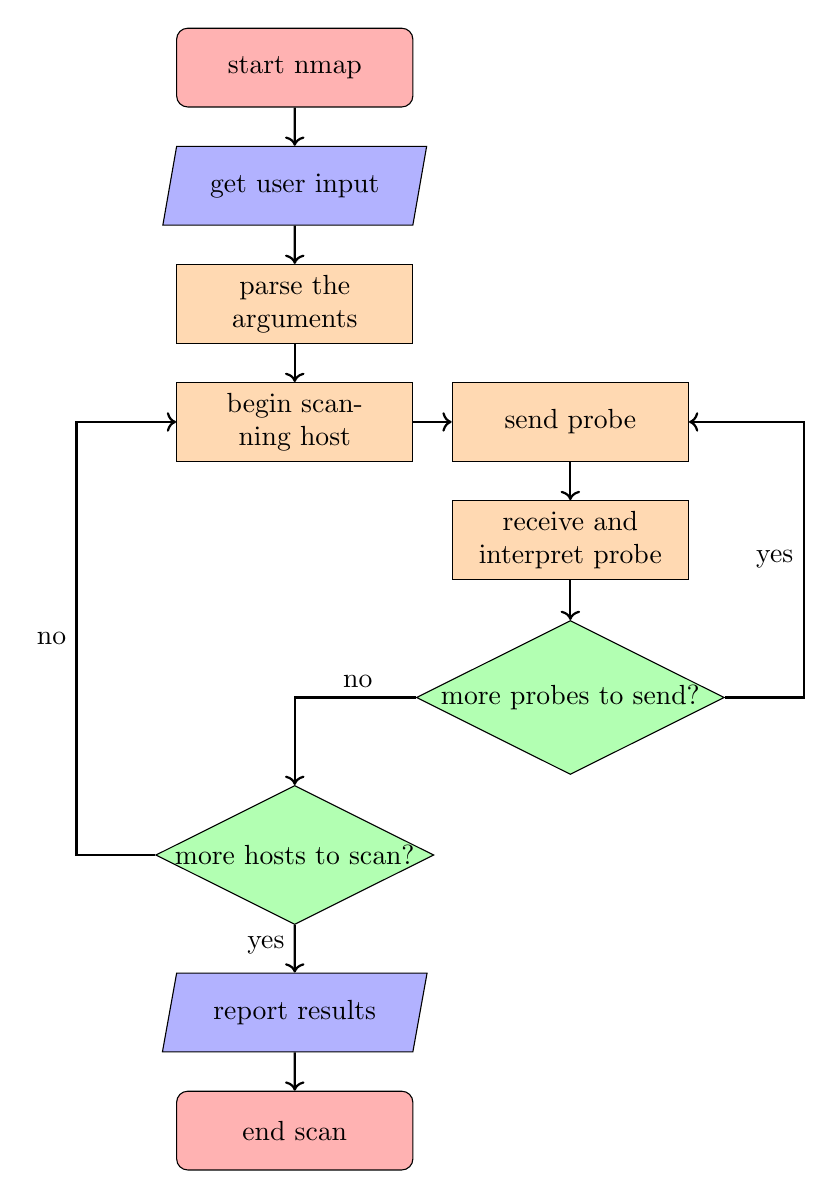
\begin{tikzpicture}[node distance=1.5cm]

    \node (start) [startstop] {start nmap};
    \node (get) [io, below of=start] {get user input};
    \node (arguments) [process, below of=get] {parse the arguments};
    \node (host) [process, below of=arguments] {begin scanning host};
    \node (probe) [process, right of=host, xshift=2cm] {send probe};
    \node (response) [process, below of=probe] {receive and interpret probe};
    \node (probes) [decision, below of=response, yshift=-0.5cm] {more probes to send?};
    \node (hosts) [decision, left of=probes, below of=probes, xshift=-2cm, yshift=-0.5cm] {more hosts to scan?};
    \node (report) [io, below of=hosts, yshift=-0.5cm] {report results};
    \node (end) [startstop, below of=report] {end scan};

    \draw [arrow] (start) -- (get);
    \draw [arrow] (get) -- (arguments);
    \draw [arrow] (arguments) -- (host);
    \draw [arrow] (host) -- (probe);
    \draw [arrow] (probe) -- (response);
    \draw [arrow] (response) -- (probes);
    \draw [arrow] (probes) -- ([xshift=1cm]probes.east) node[anchor=east,yshift=1.75cm] {yes} |- (probe.east);
    \draw [arrow] (probes) -| node[anchor=south,xshift=0.8cm] {no} (hosts);
    \draw [arrow] (hosts) -- ([xshift=-1cm]hosts.west) node[anchor=east,yshift=2.75cm] {no} |- (host);
    \draw [arrow] (hosts) node[left, yshift=-1.15cm] {yes} -- (report);
    \draw [arrow] (report) -- (end);

  \end{tikzpicture}

  \end{framed}

  \caption{\textit{%
    A flow chart showing how nmap does scanning.
}}\label{nmapflow}

\end{figure}

The following paragraphs discuss an example nmap scan I did on my home network
I did for this project. The command I used was: \\
\verb|nmap -sC -sV -oA networkscan 192.168.1.0/24|.
The purpose of the command line flags was to enable script scanning \verb|-sc|,
enable version detection \verb|-sV|,
and then output all results in all the common formats:
XML, nmap and greppable, using the base name \verb|networkscan|.
The program outputs to three files: \verb|networkscan.(nmap,gnmap,xml)|.
Before I go into what each file contains, I will explain some terminology: something is greppable if it can be
easily searched with the Linux utility \verb|grep|\cite{man:grep}.
Grep stands for Globally search a Regular Expression and Print,
which instructs the computer to search the specified file for lines that contain a certain word or pattern;
for example, the command to find all lines with the word ``hi'' in them in the file ``document'' would be
\verb|grep `hi' document|.

Returning to the files nmap created: \verb|networkscan.nmap| contains what would usually
be printed by nmap, while the scan is being run.
It looks like this:
\begin{verbatim}
# Nmap 7.70 scan initiated Wed Apr 10 19:36:18 2019 as:
    nmap -sC -sV -oA /home/tritoke/thing 192.168.1.0/24
Nmap scan report for router.asus.com (192.168.1.1)
Host is up (1.0s latency).
Not shown: 995 closed ports
PORT     STATE SERVICE    VERSION
53/tcp   open  domain     (generic dns response: NOTIMP)
| fingerprint-strings: 
|   DNSVersionBindReqTCP: 
|     version
|_    bind
80/tcp   open  http       ASUS WRT http admin
|_http-server-header: httpd/2.0
|_http-title: Site doesn't have a title (text/html).
515/tcp  open  printer
8443/tcp open  ssl/http   ASUS WRT http admin
|_http-server-header: httpd/2.0
|_http-title: Site doesn't have a title (text/html).
| ssl-cert: Subject: commonName=192.168.1.1/countryName=US
| Not valid before: 2018-05-05T05:05:17
|_Not valid after:  2028-05-05T05:05:17
9100/tcp open  jetdirect?
1 service unrecognized despite returning data.
  If you know the service/version,
please submit the following fingerprint at
https://nmap.org/cgi-bin/submit.cgi?new-service :
SF-Port53-TCP:V=7.70%I=7%D=4/10%Time=5CAE3DC5%P=x86_64-pc-Linux
-gnu%r(DNSVSF:ersionBindReqTCP,20,"\0\x1e\0\x06\x85\x85\0\x01\0 
\0\0\0\0\0\x07version\SF:x04bind\0\0\x10\0\x03")%r(DNSStatusReq
uestTCP,E,"\0\x0c\0\0\x90\x04\0\0SF:\0\0\0\0\0\0");
Service Info: CPE: cpe:/o:asus:wrt_firmware
\end{verbatim}
The above is the report for only one device on the network.
In it, you can see information such as which ports are open, and what services are running behind them.
As this example device is network router, you can see port 8443, which nmap has recognised to be hosting
the ASUS web admin, from which you can configure the router.
There follows some other associated information extracted from the server.
Most of this extra information is derived from the \verb|-sC| flag,
which enables script scanning,
and allows advanced interaction with running services specifically to gain more
information by providing specialised probing per protocol. We can also see at the end an
unrecognised service. Nmap shows us the data it returned and asks us to submit a new service
report at a given URL if we recognise the service. This system of submitting fingerprints of
services explains why nmap is so good at recognising services: it has a lot of data to look at and learn
from in regards to service fingerprinting.

\verb|Networkscan.gnmap| contains exactly the same information as \\
\verb|networkscan.nmap|,
but the output is formatted to enable easy searching with the grep utility.
I reproduce part of the output file below:
\begin{verbatim}
# Nmap 7.70 scan initiated Wed Apr 10 19:36:18 2019 as:
    nmap -sC -sV -oA /home/tritoke/networkscan 192.168.1.0/24
Host: 192.168.1.1 (router.asus.com) Status:
Host: 192.168.1.1 (router.asus.com) Ports: 53/open/tcp//domain//
      (generic dns response: NOTIMP)/, 80/open/tcp//http//ASUS
      WRT http admin/,515/open/tcp//printer///,
      8443/open/tcp//ssl| http//ASUS WRT http
      admin/,9100/open/tcp//jetdirect?///
      Ignored State: closed (995)
Host: 192.168.1.8 (android-25a97e36c2e74456)  Status: Up
Host: 192.168.1.8 (android-25a97e36c2e74456)  Ports: 5060/
      filtered/tcp//sip/// Ignored State: closed (999)
\end{verbatim}
As you can see above, all of the information is on a single line for each type of scan.
This is useful: for example, if you want to scan a large number of hosts and just want
to know which hosts are up you could use \\
\verb|grep `Status: Up' networkscan.gnmap|
which outputs this:
\begin{verbatim}
$ grep `Status: Up' networkscan.gnmap
Host: 192.168.1.1 (router.asus.com) Status: Up
Host: 192.168.1.8 (android-25a97e36c2e74456) Status: Up
Host: 192.168.1.10 (diskstation) Status: Up
Host: 192.168.1.88 () Status: Up
Host: 192.168.1.88 () Status: Up
Host: 192.168.1.117 () Status: Up
Host: 192.168.1.159 (groot) Status: Up
Host: 192.168.1.159 (groot) Status: Up
Host: 192.168.1.176 (ET0021B7C01F2E) Status: Up
\end{verbatim}
This shows the hosts which are online and their host names. Other ways to use the greppable
output format would be to search for which ports are open on only one machine, or which hosts have a
webserver running on them or a vulnerable version of a mail server etc. In general, the \verb|.gnmap|
output is useful for when you want to use grep to filter results.

Finally, we have the \gls{xml} format file, \\
\verb|networkscan.xml| part of which is reproduced below:
\lstset{language=xml}
\begin{lstlisting}
<?xml version="1.0" encoding="UTF-8"?>
<!DOCTYPE nmaprun>
<?xml-stylesheet href="file:///usr/bin/../share/nmap/nmap.xsl" type="text/xsl"?>
<!-- Nmap 7.70 scan initiated Wed Apr 10 19:36:18 2019 as: nmap -sC -sV -oA /home/tritoke/thing 192.168.1.0/24 -->
<nmaprun scanner="nmap" args="nmap -sC -sV -oA /home/tritoke/thing 192.168.1.0/24" start="1554921378" startstr="Wed Apr 10 19:36:18 2019" version="7.70" xmloutputversion="1.04">
<verbose level="0"/>
<debugging level="0"/>
<host starttime="1554921379" endtime="1554923187"><status state="up" reason="syn-ack" reason_ttl="0"/>
<address addr="192.168.1.1" addrtype="ipv4"/>
<hostnames>
<hostname name="router.asus.com" type="PTR"/>
</hostnames>
<ports><extraports state="closed" count="995">
<extrareasons reason="conn-refused" count="995"/>
</extraports>
<port protocol="tcp" portid="53"><state state="open" reason="syn-ack" reason_ttl="0"/><service name="domain" extrainfo="generic dns response: NOTIMP" servicefp="SF-Port53-TCP:V=7.70%I=7%D=4/10%Time=5CAE3DC5%P=x86_64
-pc-Linux-gnu%r(DNSVersionBindReqTCP,20,&quot;\0\x1e\0\x06\x85\x85\0
\x01\0\0\0\0\0\0\x07version\x04bind\0\0\x10\0\x03&quot;)%r
(DNSStatusRequestTCP,E,&quot;\0\x0c\0\0\x90\x04\0\0\0\0\0\0\0\0&quot;);" method="probed" conf="10"/><script id="fingerprint-strings" output="&#xa;  DNSVersionBindReqTCP: &#xa;    version&#xa;    bind"><elem key="DNSVersionBindReqTCP">&#xa;    version&#xa;    bind</elem>
</script></port>
\end{lstlisting}
It can be seen that this file is extremely verbose.
It contains the reason why each port has the state it does, as well as a
vast amount of other data that the other scans did not include. 
The consequence is that this output format is not very easy for humans to read,
meaning that this format is available because it is easier for other programs
to parse than the other formats. As well as this the extra information can be good
if you really need to dive into why a port was marked as closed etc.\
or the exact bytes that a service replied with.

In terms of where nmap lives in the software stack, it is an application at level 7 when the
user interacts, with it but uses several libraries that interact at level 2, which it uses to get
the raw headers of the packets being sent and thus gain information from them (see Figure~\ref{nmapblock}).
Nmap has virtually no competitors in the Linux ecosystem,
other than possibly Angry IP Scanner,
which is another open source network scanner,
except it has a much smaller user base. \\

\begin{figure}[H]

  \begin{framed}

  \centering
  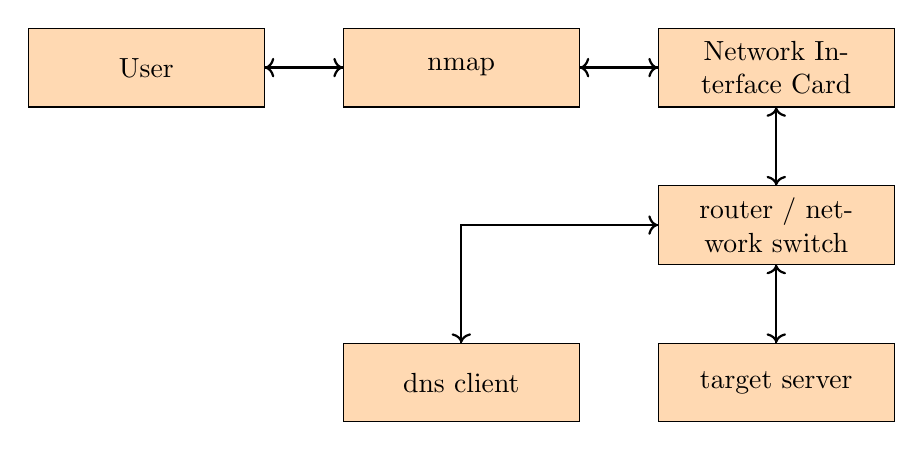
\begin{tikzpicture}[node distance=2cm]

    \node (user) [process] {User};
    \node (nmap) [process, right of=user, xshift=2cm] {nmap};
    \node (nic) [process, right of=nmap, xshift=2cm] {Network Interface Card};
    \node (router) [process, below of=nic] {router / network switch};
    \node (target) [process, below of=router] {target server};
    \node (dnsserver) [process, left of=target, xshift=-2cm] {\gls{dns} client};

    \draw [arrow] (nic) -- (router);
    \draw [arrow] (router) -- (nic);
    \draw [arrow] (target) -- (router);
    \draw [arrow] (router) -- (target);
    \draw [arrow] (dnsserver) |- (router);
    \draw [arrow] (router) -| (dnsserver);
    \draw [arrow] (nic) -- (nmap);
    \draw [arrow] (nmap) -- (nic);
    \draw [arrow] (user) -- (nmap);
    \draw [arrow] (nmap) -- (user);

  \end{tikzpicture}

  \end{framed}

  \caption{\textit{%
    A block diagram showing how nmap sits in the software stack.
}}\label{nmapblock}

\end{figure}

Before describing my program in detail I would like to explain some terminology I will use:
``parse the arguments'' means taking the string of text that the user enters after the program name i.e. 
\verb|program <text>|. It is these texts that represent the arguments. Parsing the arguments
means turning those strings into useful information that the program can use.
For example, my program will allow people to enter the port number(s) they want to scan.
I want them to be able to do this by specifying a range of ports.
If the user specifies \verb|10-20|, this would mean ports 10, 11, \ldots, 20.
Thus an example of parsing would be the turning of \verb|10-20| into the list of numbers
from 10 to 20 as shown in Algorithm~\ref{argumentparsing} below.
``Probes'' refer to the actual packets being sent to the server;
I will refer to anything sent from my code to another machine as being a ``probe''.
I will use the term ``hosts'' to mean the other machines on the network that we are scanning.

\begin{algorithm}
  \caption{\textit{%
    This is an example algorithm for parsing the port range argument I gave
    as an example above, extended by allowing for comma separated lists
    of ports intermixed with ranges.
}}\label{argumentparsing}
  \begin{algorithmic}[1]
    \Procedure{port parser}{}
    \State{$\textit{argument} \gets \text{string after program name}$}
    \State{$\textit{chunks} \gets \text{argument split on `,'}$}
    \State{$\textit{ports} \gets \text{empty list}$}
    \For{\textit{chunk} in \textit{chunks}}
      \If{\textit{chunk} contains ``-''}\Comment{a range chunk}
        \State{$\textit{numbers} \gets \text{\textit{chunk} split on ``-''}$}
        \For{$\textit{port} \gets \text{\textit{numbers}[0],\textit{numbers}[1]}$}
          \State{Append \textit{port} to \textit{ports}}
        \EndFor{}
      \Else{}\Comment{a single number chunk}
        \State{Append \textit{chunk} to \textit{ports}}
      \EndIf{}
    \EndFor{}
    \Return{\textit{ports}}
    \EndProcedure{}
  \end{algorithmic}
\end{algorithm}

\subsection{Prospective Users}

The prospective users of my program would be system administrators, penetration testers or network
engineers. In my particular case, prospective users would be my school's system administrators.
It would allow them to see an outsider's perspective on,
for example, the \gls{server} running the school's website page,
or to see if any of the programs on the \glspl{server} were leaking information
through \glspl{banner} etc.
Banners are short strings of text which a service or program will send to identify itself when
it receives a new connection. They often contain information such as protocol version etc., which
allows the connecting client to know how to communicate with the service. However, they can also
reveal too much information, such as the version number of the service running. 
If the service version is old, then it is likely that bugs will have been found in that version 
of the program.
This information could allow an attacker to gain access to the server by exploiting the vulnerability
in that service. This can obviously be prevented by keeping services up to date; however, that
is not always possible, so as a best practice banners should reveal the minimum amount of information
possible such that the client can interact with the service.

I plan to use my school's system administrators users in order to gain some feedback
as to the usability and performance of my program.

\subsection{Data Dictionary}

While my program is running it will need to store many different things in memory:
\begin{itemize}
  \item{The list of hosts to scan}
  \item{The list of ports to scan on each host}
  \item{The state of each port we are scanning on each host}
  \item{The packet received by the listening socket (temporarily before processing)}
  \item{The probes to be used for version detection}
\end{itemize}
I am going to try to estimate the amount of RAM my program will use, based on scanning a 
\gls{cidr}-specified subnet of 192.168.1.0/24, and the most common 1000 ports of each machine.
For the purpose of RAM estimation I will not consider version detection, as I am unsure of how I will implement it currently.
To measure the size of an object in Python we can use the \verb|getsizeof| function provided by the
\verb|sys| module. I also have a file called `hosts' which contains the addresses specified by
192.168.1.0/24 and a file `ping\_bytes' which contains 4 captured packets from the ping command
which I captured during an early exploratory testing phase.
\lstset{language=Python}
\begin{lstlisting}[label=testingsize,caption=\textit{Some testing I did on the size of Python objects.}]
>>> with open("hosts", "r") as f
...     hosts = f.read().splitlines()
... 
>>> import sys
>>> sys.getsizeof(hosts)
2216
>>> ports = list(range(1000))
>>> sys.getsizeof(ports)
9112
>>> len(hosts)*sys.getsizeof(ports) / 2**10  # 2*10 is one kibibyte
2278.0
>>> sys.getsizeof(True)
28
>>> len(hosts)*(sys.getsizeof(True)) / 2**10
7.0
>>> pings[0]
'45 00 00 54 0f 82 40 00 40 01 2d 25 7f 00 00 01 7f 00 00 01 08 00 41 c5 02 4f 00 01 cd ef 0f 5c de 9b 0d 00 08 09 0a 0b 0c 0d 0e 0f 10 11 12 13 14 15 16 17 18 19 1a 1b 1c 1d 1e 1f 20 21 22 23 24 25 26 27 28 29 2a 2b 2c 2d 2e 2f 30 31 32 33 34 35 36 37'
>>> from binascii import unhexlify
>>> ping = unhexlify(pings[0].replace(" ", ""))  # turn the string of numbers into a bytes object
>>> sys.getsizeof(ping)
117
>>> len(hosts)*sys.getsizeof(ping) / 2**10
29.25
>>> 2278.0 + 7.0 + 29.25 + 2.22
2316.47
\end{lstlisting}
As shown above in Listing~\ref{testingsize}, we can see that by far the most space intensive item stored
by our program will be the port numbers for each host, making up just over than ninety eight percent
of the total space used by the mock data I created. However, a total of 2.3 mebibytes is not a huge
amount of data by any means.

\begin{center}
  \begin{tabular}{p{3cm} l r r}
    \toprule
    Holding    & Data type   & Space used /Kib & Percentage of total \\
    \midrule
    ports      & List[int]   & 2278            & 98.34 \\
    hosts      & List[str]   & 2.22            & 0.1   \\
    port state & List[bool]  & 7               & 0.3   \\
    packets    & List[bytes] & 29.25           & 1.26  \\
    \bottomrule
  \end{tabular}
\end{center}

\subsection{Data Flow Diagram}

In my application there will be three-way information flow: 
\begin{enumerate}
  \item{Sending packets out from my application}
  \item{Receiving packets back from the targets}
  \item{Transferring data between functions}
\end{enumerate}
My program will only hold information in memory and provides no utility
for saving the information from scans. This is because on the target systems
(Linux/Unix based machines), the shell which is used to run commands has
a very simple way of placing output in files by use of
Unix ``pipes'', which are how Unix-based operating systems handle interprocess
communications. 
If nmap did not have a dedicated saving utility, the following command could 
be used to save the output of nmap to a text file called outputfile: \\
\verb|nmap 192.168.1.0 > outputfile|. Thus, in my application, for the sake of
simplicity, this is the method I will use to save output.

Figure~\ref{dataflow} below shows the proposed data flow in my program.

\begin{figure}[H]
  \centering
  \begin{framed}
  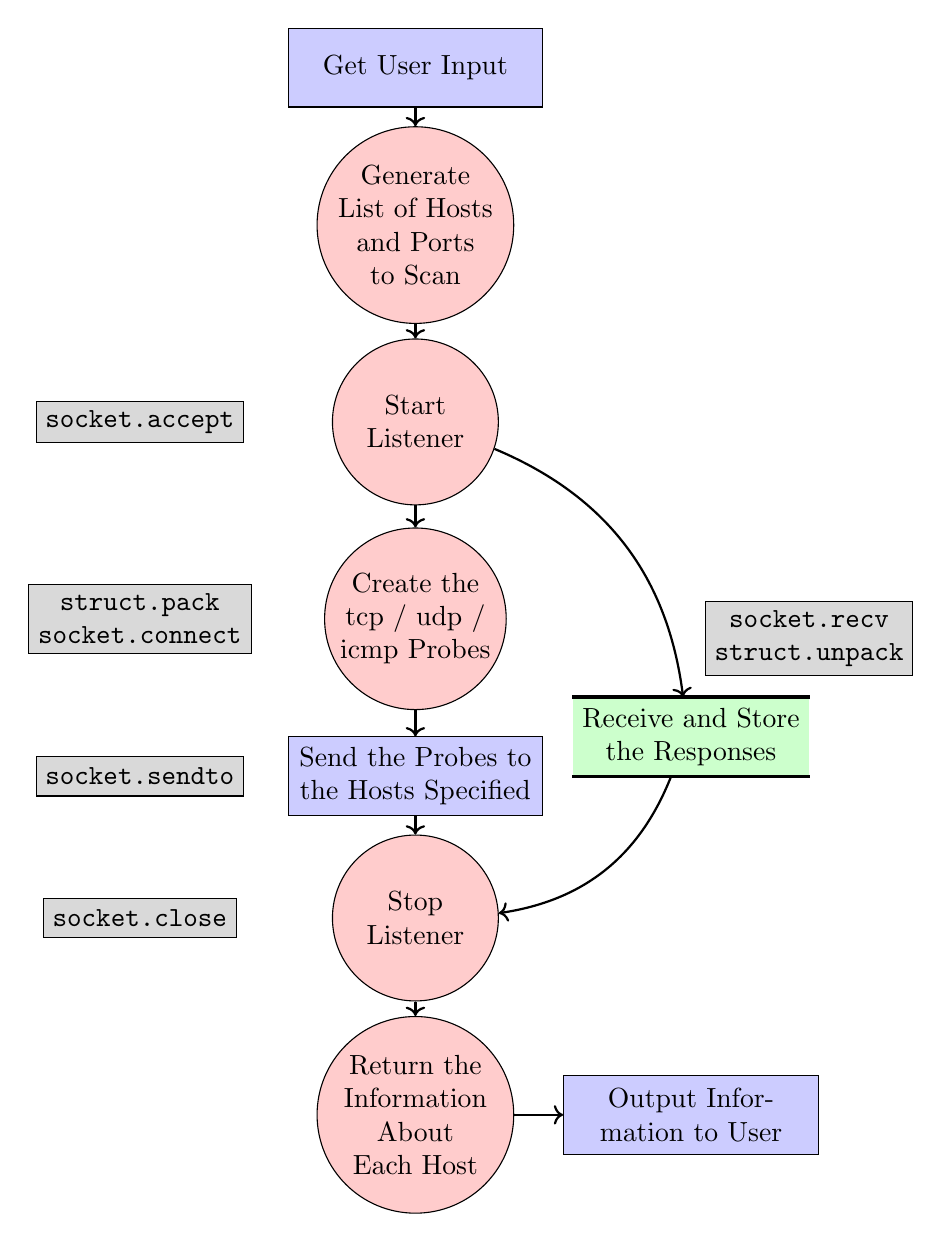
\begin{tikzpicture}[node distance=1.5cm]
    \node [inputoutput] (input) {Get User Input};
    \node [function, below of=input, yshift=-0.5cm] (hosts) {Generate List of Hosts and Ports to Scan};
    \node [function, below of=hosts, yshift=-1cm] (listen) {Start Listener};
    \node [function, below of=listen, yshift=-1cm] (create) {Create the \gls{tcp} / \gls{udp} / \gls{icmp} Probes};
    \node [inputoutput, below of=create, yshift=-0.5cm] (send) {Send the Probes to the Hosts Specified};
    \node [function, below of=send,yshift=-0.3cm] (stop) {Stop Listener};
    \node [datastore, right of=stop, xshift=2cm, yshift=2.3cm] (responses) {Receive and Store the Responses};
      \draw [black,very thick] (responses.north west) -- (responses.north east);
      \draw [black,very thick] (responses.south west) -- (responses.south east);
    \node [function, below of=stop, yshift=-1cm] (return) {Return the Information About Each Host};
    \node [inputoutput, right of=return, xshift=2cm] (finish) {Output Information to User};
    \node [method,left of=listen, xshift=-2cm] {\verb|socket.accept|};
    \node [method,left of=create, xshift=-2cm, text width=2.6cm] {\verb|struct.pack| \verb|socket.connect|};
    \node [method,left of=send, xshift=-2cm] {\verb|socket.sendto|};
    \node [method,left of=stop, xshift=-2cm] {\verb|socket.close|};
    \node [method,right of=responses,yshift=1.25cm,text width=2.4cm] {\verb|socket.recv| \verb|struct.unpack|};

    \path[arrow]{
      (input) edge node [right] {} (hosts)
      (hosts) edge node [right] {} (listen)
      (listen) edge node [right] {} (create)
      (create) edge node [right] {} (send)
      (send) edge node [right] {} (stop)
      (listen) edge[bend left] node [left] {} (responses)
      (responses) edge[bend left] node [left] {} (stop)
      (stop) edge node [right] {} (return)
      (return) edge node[bend right] [right] {} (finish)
    };
  \end{tikzpicture}
  \end{framed}
  \caption{\textit{%
    A data flow digram for information in my application.
}}\label{dataflow}
\end{figure}

\subsection{Description of Solution Details}

As already stated above on page~\pageref{pythonreason},
I will be using Python version 3.7.2 for my project because I am already familiar with Python's
syntax and its socket library has a very nice high level \gls{api} for making system calls to
the kernel's low level networking functions. This makes it ideal for a networking project
like mine, as it allows me to prototype easily, and explore many ideas about how I could implement
my solution in a time-efficient manner.

I decided to start my project by researching how to write code for receiving and sending
\gls{icmp} \verb|echo requests| (i.e.\ pings).
\gls{icmp} sits at layer 3 of the \gls{osi}.
This means that it functions at a layer below that to which you are normally given access in the socket module.
Sending an \gls{icmp} \verb|echo request| requires a raw socket.
A raw socket is one which will return everything contained by the ethernet/wifi frame, including
the raw \gls{ip} headers.
The bytes object received from a raw socket thus requires unpacking to extract relevant information.
The struct module provides a convenient \gls{api} for converting between packed values,
because there is usually a difference in endianness between the network and the local machine
which requires translation.

Interactions with the socket module are mainly through the pack and unpack functions.
For each of these functions it is necessary to provide a format specifier defining how
to unpack/pack the bytes/values. 
In Listing~\ref{echosend}, you can see an example of me using the \verb|struct.pack| function to pack
the values which comprise an \gls{icmp} \verb|echo request| into a packet and sending it the localhost
address (127.0.0.1). This program is effectively the complement to the program in
Listing~\ref{echorecv}, which uses \verb|struct.unpack| to unpack value from the received \gls{icmp}
packet before printing the fields out to the terminal. Listing~\ref{echosend} makes use of an
IP checksum function which I wrote (see Listing~\ref{checksum} below).
In Figure~\ref{echodissect}, you can see the output when I run the command
\verb|ping 127.0.0.1| which the code in Listing~\ref{echorecv} is listening for packets.

\begin{algorithm}
\begin{algorithmic}[1]
\MakeRobust{\Call}
\State{$\textit{socket} \gets \text{new ICMP socket}$}
\State{$\textit{ID} \gets \text{process ID} \And 0xFFFF$}
\State{$\textit{dummy header} \gets \Call{pack}{\text{``bbHHh''}, 8, 0, 0, \textit{ID}, 1}$}
\State{$\textit{time} \gets \Call{pack}{\Call{time}{\text{now}}}$}
\State{$\textit{data} \gets \textit{time} + \text{``A''}\times(192-\Call{length}{time})$}
\State{$\textit{checksum} \gets \Call{ipchecksum}{\textit{dummy header} + \textit{data}}$}
\State{$\textit{header} \gets \Call{pack}{\text{``bbHHh''}, 8, 0, \textit{checksum}, \textit{ID}, 1}$}
\State{$\textit{packet} \gets \textit{header} + \textit{data}$}
\State{$\Call{socket.send}{packet}$}
\end{algorithmic}
\caption{\textit{%
  The psuedocode representation of Listing~\ref{echosend}.
}}
\end{algorithm}

\begin{lstlisting}[label=echosend,caption=\textit{A prototype for sending \gls{icmp} echo request packets.}]
#!/usr/bin/Python3.7
import socket
import struct
import os
import time
import array

from os import getcwd, getpid
import sys
sys.path.append("../modules/")

import ip_utils


ICMP_ECHO_REQUEST = 8

# opens a raw socket for the ICMP protocol
ping_sock = socket.socket(socket.AF_INET, socket.SOCK_RAW, socket.IPPROTO_ICMP)
# allows manual IP header creation
# ping_sock.setsockopt(socket.SOL_IP, socket.IP_HDRINCL, 1)

ID = os.getpid() & 0xFFFF

# the two zeros are the code and the dummy checksum, the one is the sequence number
dummy_header = struct.pack("bbHHh", ICMP_ECHO_REQUEST, 0, 0, ID, 1)

data = struct.pack("d", time.time()) + bytes((192 - struct.calcsize("d")) * "A", "ascii")

checksum = ip_utils.ip_checksum(dummy_header+data)

header = struct.pack("bbHHh", ICMP_ECHO_REQUEST, 0, checksum, ID, 1)

packet = header + data

ping_sock.sendto(packet, ("127.0.0.1", 1))
\end{lstlisting}

\begin{algorithm}
\begin{algorithmic}[1]
\State{$\textit{socket} \gets \text{new ICMP socket}$}
\State{$\textit{packet} \gets \Call{socket.receive}{\text{``one packet''}}$}
\State{$\textit{data} \gets \Call{unpack}{\textit{packet}}$}
\State{$\Call{print}{\textit{data}}$}
\end{algorithmic}
\caption{\textit{%
  Psuedocode for the code in Listing~\ref{echorecv}.
}}
\end{algorithm}

\begin{lstlisting}[label=echorecv,caption=\textit{A prototype for receiving \gls{icmp} echo request packets.}]
#!/usr/bin/Python3.7

import socket
import struct
import time
from typing import List

# socket object using an IPV4 address, using only raw socket access, set ICMP protocol        
ping_sock = socket.socket(socket.AF_INET, socket.SOCK_RAW, socket.IPPROTO_ICMP)

packets: List[bytes] = []

while len(packets) < 1:
    recPacket, addr = ping_sock.recvfrom(1024)
    ip_header = recPacket[:20]
    icmp_header = recPacket[20:28]

    ip_hp_ip_v, ip_dscp_ip_ecn, ip_len, ip_id, ip_flgs_ip_off, ip_ttl, ip_p, ip_sum, ip_src, ip_dst = struct.unpack('!BBHHHBBHII', ip_header)

    hl_v = f"{ip_hp_ip_v:08b}"
    ip_v = int(hl_v[:4], 2)
    ip_hl = int(hl_v[4:], 2)
    dscp_ecn = f"{ip_dscp_ip_ecn:08b}"
    ip_dscp = int(dscp_ecn[:6], 2)
    ip_ecn = int(dscp_ecn[6:], 2)
    flgs_off = f"{ip_flgs_ip_off:016b}"
    ip_flgs = int(flgs_off[:3],2)
    ip_off = int(flgs_off[3:], 2)
    src_addr = socket.inet_ntoa(struct.pack('!I', ip_src))
    dst_addr = socket.inet_ntoa(struct.pack('!I', ip_dst))

    print("IP header:")
    print(f"Version: [{ip_v}]\nInternet Header Length: [{ip_hl}]\nDifferentiated Services Point Code: [{ip_dscp}]\nExplicit Congestion Notification: [{ip_ecn}]\nTotal Length: [{ip_len}]\nIdentification: [{ip_id:04x}]\nFlags: [{ip_flgs:03b}]\nFragment Offset: [{ip_off}]\nTime To Live: [{ip_ttl}]\nProtocol: [{ip_p}]\nHeader Checksum: [{ip_sum:04x}]\nSource Address: [{src_addr}]\nDestination Address: [{dst_addr}]\n")

    msg_type, code, checksum, p_id, sequence = struct.unpack('!bbHHh', icmp_header)
    print("ICMP header:")
    print(f"Type: [{msg_type}]\nCode: [{code}]\nChecksum: [{checksum:04x}]\nProcess ID: [{p_id:04x}]\nSequence: [{sequence}]"
    packets.append(recPacket)
open("current_packet", "w").write("\n".join(" ".join(map(lambda x: "{x:02x}", map(int, i))) for i in packets))
\end{lstlisting}

\begin{algorithm}
\begin{algorithmic}[1]
\Function{ip\_checksum}{data}{}
\If{\Call{length}{data} is odd}
\State{$\text{data.append(0)}$}
\EndIf{}
\State{$\textit{total} \gets 0$}
\For{\textit{i} in 0,2,\Call{length}{data}}
\State{$\textit{total} \gets \textit{total} + \text{\textit{data}[\textit{i}]} << 8$}
\State{$\textit{total} \gets \textit{total} + \text{\textit{data}[\textit{i}+1]}$}
\EndFor{}
\State{$\textit{carried} \gets (\textit{total} - (\text{\textit{total} \& 0xFFFF)}) >> 16$}
\State{$\textit{total} \gets \text{\textit{total} \& 0xFFFF}$}
\State{$\textit{total} \gets \textit{total} + \textit{carried}$}
\If{$\textit{total} > \text{0xFFFF}$}{}
\State{$\textit{total} \gets \text{\textit{total} \& 0xFFFF}$}
\State{$\textit{total} \gets \text{\textit{total} + 1}$}
\EndIf{}
\State{$\textit{total} \gets \Call{invert}{\textit{total}}{}$}
\Return{\textit{total}}
\EndFunction{}
\end{algorithmic}
\end{algorithm}

\begin{lstlisting}[label=checksum,caption=\textit{A function for calculating the IP checksum for a set of bytes.}]
def ip_checksum(packet: bytes) -> int:
    """
    ip_checksum function takes in a packet
    and returns the checksum.
    """
    if len(packet) % 2 == 1:
        # if the length of the packet is odd, add a NULL byte
        # to the end as padding to make it even in length
        packet += b"\0"

    total = 0
    for first, second in (
            packet[i:i+2]
            for i in range(0, len(packet), 2)
    ):
        total += (first << 8) + second

    # calculate the number of times a
    # carry bit was added and add it back on
    carried = (total - (total & 0xFFFF)) >> 16
    total &= 0xFFFF
    total += carried

    if total > 0xFFFF:
        # adding the carries generated a carry
        total &= 0xFFFF
        total += 1

    # invert the checksum and take the last 16 bits
    return (~total & 0xFFFF)
\end{lstlisting}

\begin{figure}[H]
  \centering
  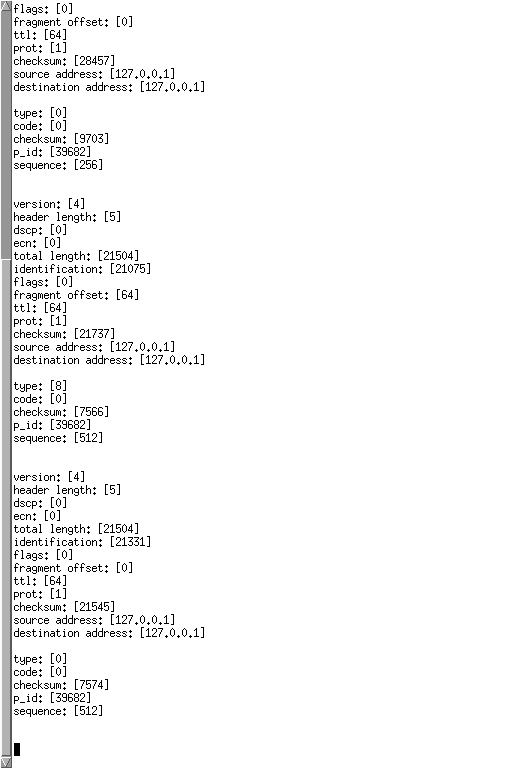
\includegraphics[width=\textwidth]{deconstructed_headers.png}
  \caption{\textit{%
    Dissecting an \gls{icmp} echo request packet.
}}\label{echodissect}
\end{figure}

\begin{figure}[H]
  \centering
  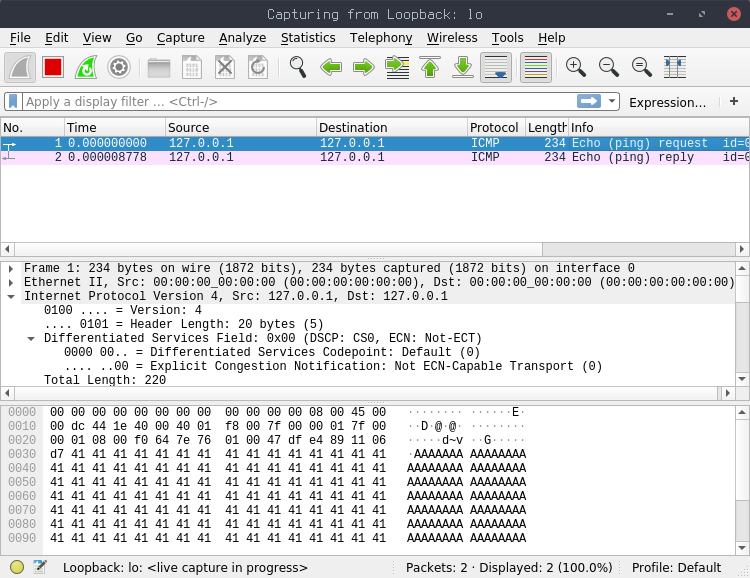
\includegraphics[width=\textwidth]{ping_send_success.png}
  \caption{\textit{%
    Screenshot of Wireshark showing a successful send of an \gls{icmp} echo request packet.
}}\label{pingsuccess}
\end{figure}

\begin{figure}[H]
  \centering
  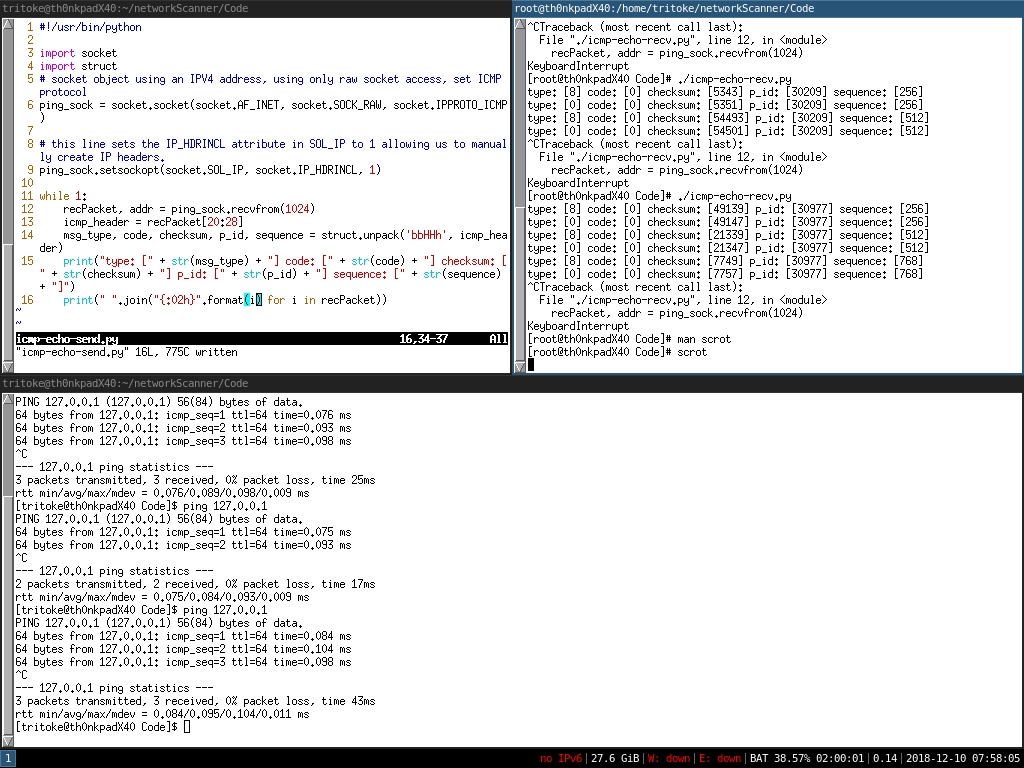
\includegraphics[width=\textwidth]{local_self_ping.png}
  \caption{\textit{%
    Screenshot showing me first successfully dissecting an \gls{icmp} echo request packet.
}}\label{dissectsuccess}
\end{figure}

Having written a prototype program which was capable of sending an \gls{icmp} \verb|echo request|
and another prototype which was capable of receiving and unpacking it.
Having done these prototypes I identified that it would be best to abstract the
code for dissecting all the headers i.e.\ \gls{icmp}, \gls{tcp} and \gls{ip} into classes
where I can just pass the received packet into the class and have the class dissect it for me.
This will also give me access to some of the benefits of classes, such as the \verb|__repr__| method,
which is called when you print classes out and allows control over what is printed out.
Before embarking on the final program,
I decided to write a prototype ping scanner,
as this would allow me to get a feel for making a scanner,
and to further exploring low level protocol interactions.

\begin{lstlisting}[label=pingscan,caption=\textit{An attempt at making a ping scanner.}]
#!/usr/bin/Python3.7
from os import getcwd, getpid
import sys
sys.path.append("../modules/")

import ip_utils

import socket
from functools import partial
from itertools import repeat
from multiprocessing import Pool
from contextlib import closing
from math import log10, floor
from typing import List, Tuple
import struct
import time


def round_significant_figures(x: float, n: int) -> float:
    """
    rounds x to n significant figures.
    round_significant_figures(1234, 2) = 1200.0
    """
    return round(x, n-(1+int(floor(log10(abs(x))))))


def recieved_ping_from_addresses(ID: int, timeout: float) -> List[Tuple[str, float, int]]:
    """
    Takes in a process id and a timeout and returns the list of addresses which sent
    ICMP ECHO REPLY packets with the packed id matching ID in the time given by timeout.
    """
    ping_sock = socket.socket(socket.AF_INET, socket.SOCK_RAW, socket.IPPROTO_ICMP)
    time_remaining = timeout
    addresses = []
    while True:
        time_waiting = ip_utils.wait_for_socket(ping_sock, time_remaining)
        if time_waiting == -1:
            break
        time_recieved = time.time()
        recPacket, addr = ping_sock.recvfrom(1024)
        ip_header = recPacket[:20]
        ip_hp_ip_v, ip_dscp_ip_ecn, ip_len, ip_id, ip_flgs_ip_off, ip_ttl, ip_p, ip_sum, ip_src, ip_dst = struct.unpack('!BBHHHBBHII', ip_header)
        icmp_header = recPacket[20:28]
        msg_type, code, checksum, p_id, sequence = struct.unpack('bbHHh', icmp_header)
        time_remaining -= time_waiting
        time_sent = struct.unpack("d", recPacket[28:28+struct.calcsize("d")])[0]
        time_taken = time_recieved - time_sent
        if p_id == ID:
            addresses.append((str(addr[0]), float(time_taken), int(ip_ttl)))
        elif time_remaining <= 0:
            break
        else:
            continue
    return addresses


with closing(socket.socket(socket.AF_INET, socket.SOCK_RAW, socket.IPPROTO_ICMP)) as ping_sock:
    addresses = ip_utils.ip_range("192.168.1.0/24")
    local_ip = ip_utils.get_local_ip()
    if addresses is not None:
        addresses_to_scan = filter(lambda x: x!=local_ip, addresses)
    else:
        print("error with ip range specification")
        exit()
    p = Pool(1)
    ID = getpid()&0xFFFF
    replied = p.apply_async(recieved_ping_from_addresses, (ID, 2))
    for address in zip(addresses_to_scan, repeat(1)):
        try:
            packet = ip_utils.make_icmp_packet(ID)
            ping_sock.sendto(packet, address)
        except PermissionError:
            pass
    p.close()
    p.join()
    hosts_up = replied.get()
    print("\n".join(map(lambda x: f"host: [{x[0]}]\tresponded to an ICMP ECHO REQUEST in {round_significant_figures(x[1], 2):<10} seconds, ttl: [{x[2]}]", hosts_up)))
\end{lstlisting}

\begin{figure}[H]
  \centering
  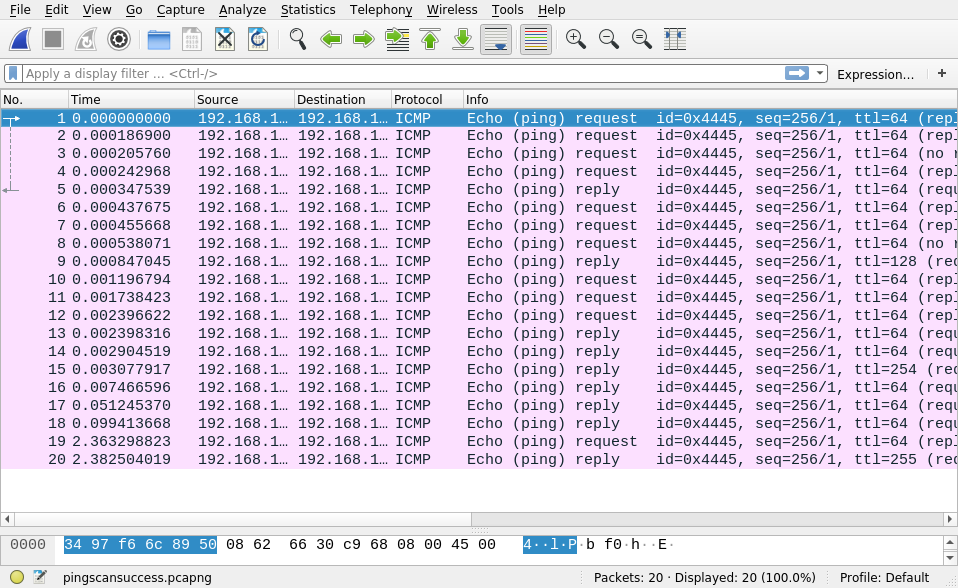
\includegraphics[width=\textwidth]{pingscan.png}
  \caption{\textit{%
    Screenshot of Wireshark showing a successful ping scan.
}}\label{pingscansuccess}
\end{figure}

\lstset{language=C}
\begin{lstlisting}[label=pingscanout,caption=\textit{The output of from the ping scanner on the run which generated the \gls{pcap} file in figure~\ref{pingscansuccess}}]
$ sudo ./ping_scan.py
host: [192.168.1.1]	responded to an ICMP ECHO REQUEST in 0.00037    seconds, ttl: [64]
host: [192.168.1.35] responded to an ICMP ECHO REQUEST in 0.00042    seconds, ttl: [128]
host: [192.168.1.37] responded to an ICMP ECHO REQUEST in 0.002      seconds, ttl: [64]
host: [192.168.1.117] responded to an ICMP ECHO REQUEST in 0.0017     seconds, ttl: [64]
host: [192.168.1.176] responded to an ICMP ECHO REQUEST in 0.0014     seconds, ttl: [254]
host: [192.168.1.14] responded to an ICMP ECHO REQUEST in 0.0072     seconds, ttl: [64]
host: [192.168.1.246] responded to an ICMP ECHO REQUEST in 0.049      seconds, ttl: [64]
host: [192.168.1.8] responded to an ICMP ECHO REQUEST in 0.099      seconds, ttl: [64]
\end{lstlisting}

Completion of these prototypes has given me an understanding of how I will structure the rest of
my scanners, how to interact with Python's socket programming interface and how I can use the
struct module to make and dissect packets. My general plan for the scanners will be to start
a process that listens for responses for a set amount of time and then starts sending the packets
in a different process, before waiting for the listening process to get all the responses back and
collecting the results from that process.

\subsection{Acceptable Limitations}

My original concept included dedicated operating system detection as an option.
However, if I find that time is short having implemented version detection, it will
be an acceptable limitation to omit operating system detection.
This is because version detection can provide some indication of the operating system
in use, by virtue of the fact that some services are restricted to certain operating systems.
For example, if the scanner detected that the service ActiveSync was in use,
this would indicate that the system being scanned was a Windows system,
which is reflected in the match directive and attached CPE information for ActiveSync:
\begin{verbatim}
match activesync m|^.\0\x01\0[^\0]\0[^\0]\0[^\0]\0[^\0]\0[^\0]\0.
*\0\0\0$|s p/Microsoft ActiveSync/ o/Windows/ cpe:/a:microsoft:ac
tivesync/ cpe:/o:microsoft:windows/a
\end{verbatim}

\subsection{Test Strategy}

I am going to use two different methods to test my program:
\begin{enumerate}
\item{Unit testing}
\item{Wireshark}
\end{enumerate}
I will employ two separate testing strategies because they are good at different things,
both of which I need in order to show that my project works. First, I will use unit testing to test
some general purpose functions, which are pure functions (are independent of the current state
of the machine). 

I will use Wireshark to test those parts of the program which involve
the use of impure functions and low level networking.
Wireshark makes this easy by allowing capture of all the \glspl{pkt} going over the wire.
As well as this, it has a vast array of \gls{pkt} decoders (2231 in 
my install), which it can use to dissect almost any \gls{pkt} that is on the network.
Wireshark will allow me to see my scanners sending packets, and to check
whether the parsers I have written for the various protocol are working.
I can also check that the \glspl{csum} in each of the various protocols are valid
as Wireshark is capable of performing \gls{csum} verification for a wide variety of protocols. 

I will be running these tests on my laptop, which is a Thinkpad T480 running Arch Linux
with kernel version 5.0.7. I have installed the following versions of each of the programs
I will be using to test my code: Wireshark 3.1.0, Python 3.7.2 and PyTest 4.3.1.
I am also using pyenv version 1.2.9 to manage the version of Python in
my Python environment. I plan not to use any modules outside of the Python standard library,
so that my program is as portable as possible and its functionality is as reproducible as possible.

\section{Design}

\subsection{Overall System Design (High Level Overview)}

There are two types of scanning implemented for different scan types in my program.
\begin{itemize}
  \item{\verb|Connect()|}
  \item{Version}
  \item{Listener / Sender}
\end{itemize}
\verb|Connect()| scanning is the simplest, in that it takes in a list of \glspl{port} and simply 
calls \verb|socket.connect| it and sees whether it can connect or not.
The \glspl{port} are marked accordingly as open or closed. 

Version scanning is very similar to \verb|Connect()| scanning in that it takes in a list of 
\glspl{port} and connects to them, except it then sends a probe to the target to elicit a response 
and gain some information about the \gls{service} running behind the \gls{port}.

Listener / sender scanning does exactly what it says on the tin: it sets up a ``listener'' in 
another process to listen for responses from the host which the ``sender'' is sending \glspl{pkt} 
to. It can then differentiate between open, open|filtered, filtered and closed \glspl{port},
based on whether it receives a \gls{pkt} back and what flags are set in the received \gls{pkt}. 
Flags are parts of \gls{tcp} \glspl{pkt} that constitute a one byte long section,
which store ``flags'' where each bit in the byte represents a different flag.

\subsection{Design of User Interface}

I am designing my system to have a similar interface to the most common tool currently used: nmap.
This is because I believe that having a familiar interface will not only make it easier for someone 
who is familiar with nmap to use my tool, it also has the advantage that anything learnt using either tool 
is applicable to both, which benefits everyone.

Based on this perception, I plan to use the same option flags as nmap, as well as similar help messages 
and an almost identical call signature (how the program is used on the command line). \\
Running \verb|./netscan.py <options> <target specification>| should be almost identical to
\verb|nmap <options> <target specification>| in terms of which scan types will be run, which hosts
will be scanned and which \glspl{port} are 
scanned. Below, you can see a concept help message, for my program with all the arguments I plan to
implement.

\begin{verbatim}
usage: netscan.py <options> <target specification>

required arguments:     target specification

optional arguments:     -h, --help -Pn, -sL, -sn, -sS,
                        -sT, -sU, -sV, -p, --ports, -O
                        --exclude_ports

\end{verbatim}

The above shows clearly which are required arguments, and which are optional ones.
It also shows that some some arguments can be called with either
a short format e.g.\ \verb|-p| or with a more verbose format \verb|--ports|.
This allows the user to be clearer if they are using the tool as part of an automated
script to perform scanning, as it should easier to recall the function of the more verbose flags.
If the user enters erroneous data, they should be greeted by a ValueError,
which will explain exactly what the issue was with their input, and will print out the
argument that caused the error.

\subsection{System Algorithms}

\begin{figure}[H]
  \centering
  \begin{framed}
    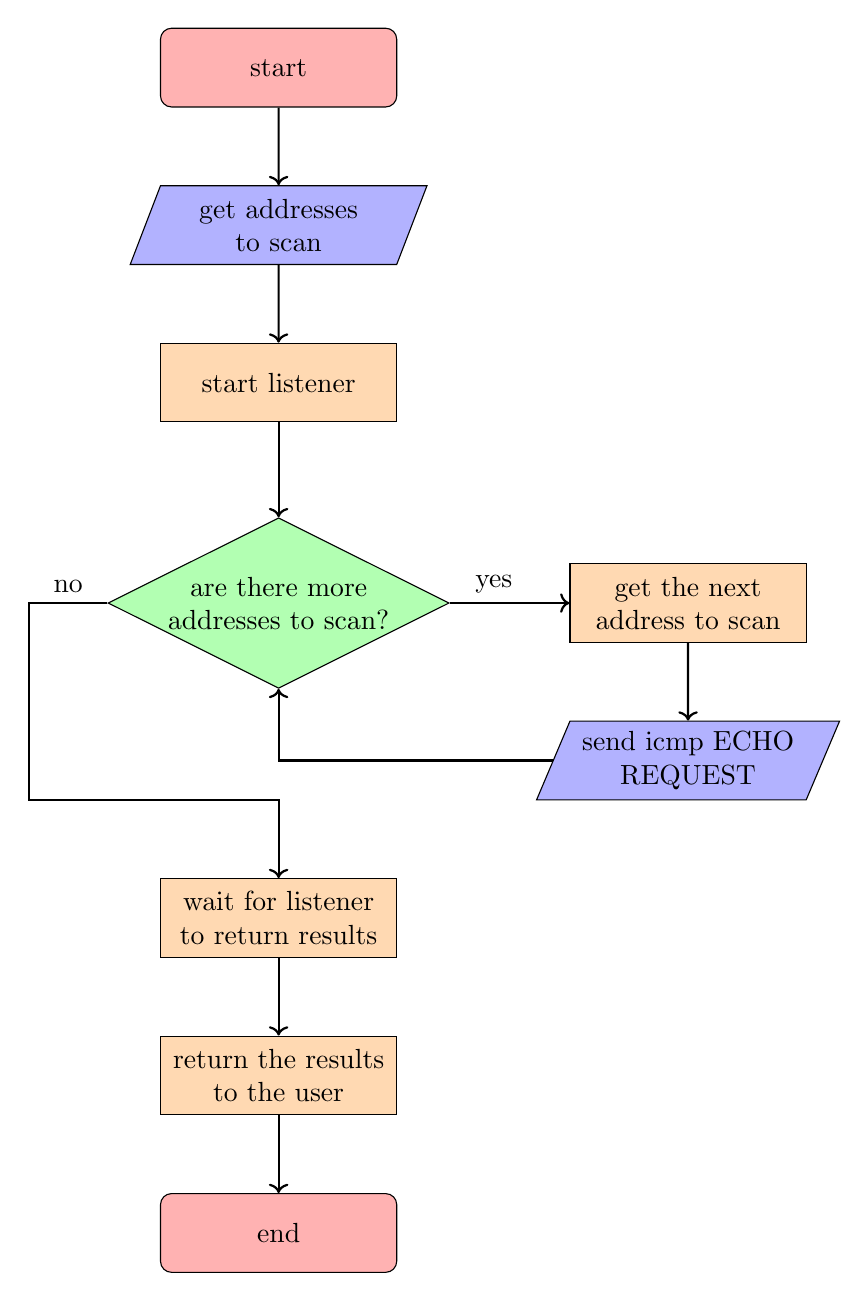
\begin{tikzpicture}[node distance=2cm]
      \node [startstop] (start) {start};
      \node [io, below of=start, text width=3cm] (input) {get addresses to scan};
      \node [process, below of=input] (listener) {start listener};
      \node [decision, below of=listener, text width=3cm, yshift=-0.8cm] (loop) {are there more addresses to scan?};
      \node [process, right of=loop, xshift=3.2cm] (get) {get the next address to scan};
      \node [io, below of=get, text width=3cm] (send) {send \gls{icmp} ECHO REQUEST};
      \node [process, below of=loop, yshift=-2cm] (wait) {wait for listener to return results};
      \node [process, below of=wait] (output) {return the results to the user};
      \node [startstop, below of=output] (end) {end};

      \draw [arrow] (start) -- (input);
      \draw [arrow] (input) -- (listener);
      \draw [arrow] (listener) -- (loop);
      \draw [arrow] (loop) -- node[midway,above,xshift=-0.2cm] {yes} (get);
      \draw [arrow] (get) -- (send);
      \draw [arrow] (send) -| node[midway,above,xshift=2cm] {} (loop);
      \draw [arrow] (loop) -- ([xshift=-1cm]loop.west) node[above,xshift=0.5cm] {no} -- ([xshift=-1cm,yshift=-2.5cm]loop.west) -| (wait);
      \draw [arrow] (wait) -- (output);
      \draw [arrow] (output) -- (end);

    \end{tikzpicture}
  \end{framed}
  \caption{\textit{%
    The logic for how I will do Ping Scanning.
}}\label{pingscanflow}
\end{figure}

\begin{figure}[H]
  \centering
  \begin{framed}
    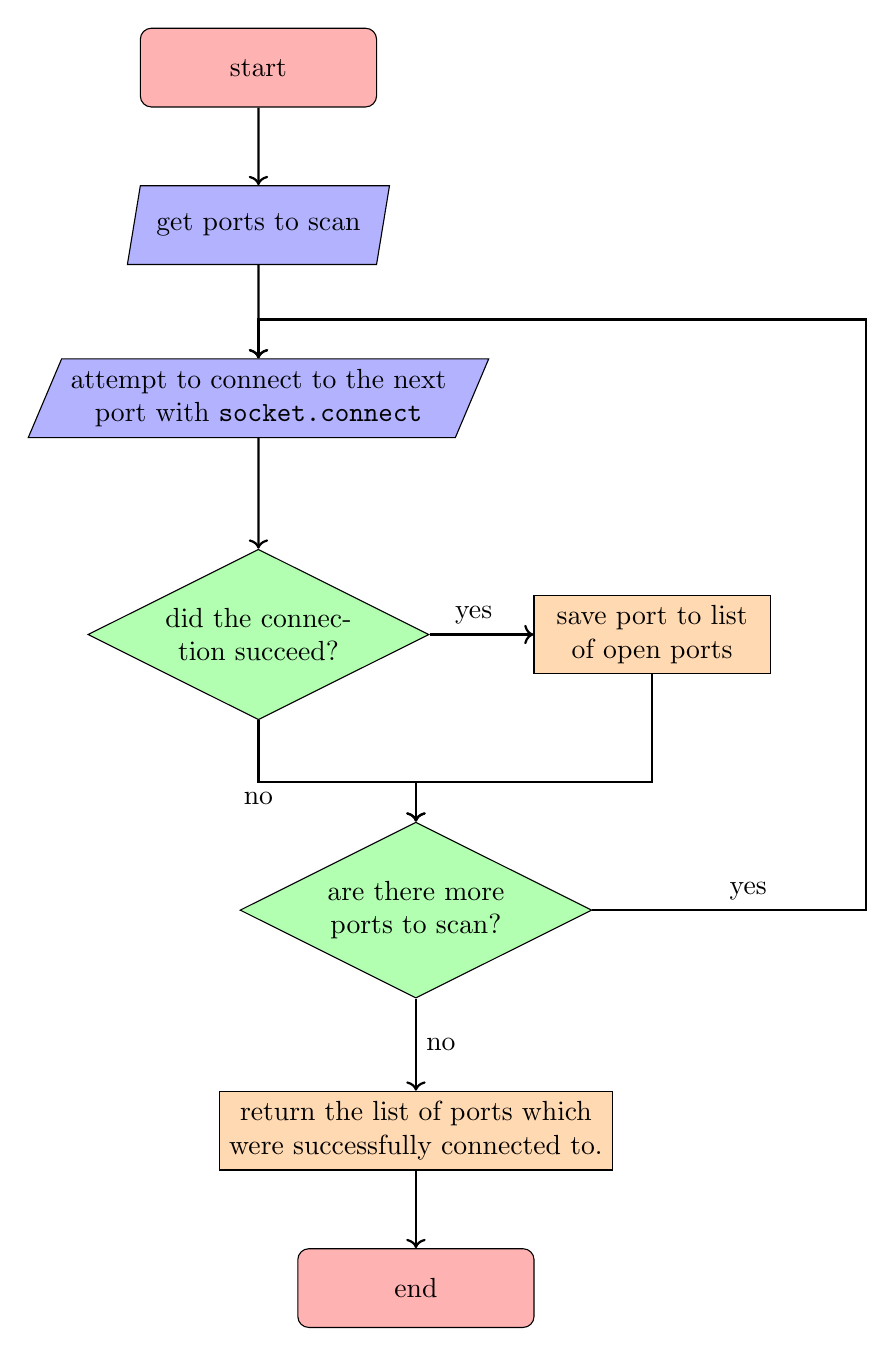
\begin{tikzpicture}[node distance=2cm]
      \node [startstop] (start) {start};
      \node [io, below of=start] (get) {get ports to scan};
      \node [io, below of=get, text width = 5cm,yshift=-0.2cm] (connect) {attempt to connect to the next port with \verb|socket.connect|};
      \node [decision, below of=connect, text width=3cm, yshift=-1cm] (save) {did the connection succeed?};
      \node [process, right of=save, xshift=3cm] (add) {save port to list of open ports};
      \node [decision, below of=save, text width=3cm, yshift=-1.5cm, xshift=2cm] (loop) {are there more ports to scan?};
      \node [process, below of=loop, yshift=-0.8cm, text width=5cm] (return) {return the list of ports which were successfully connected to.};
      \node [startstop, below of=return] (end) {end};

      \draw [arrow] (start) -- (get);
      \draw [arrow] (get) -- (connect);
      \draw [arrow] (connect) -- (save);
      \draw [arrow] (save) -- node[midway,above,xshift=-0.1cm] {yes} (add);
      \draw [arrow] (save) |- node[midway, below] {no} ([yshift=0.5cm]loop.north) -- (loop);
      \draw [arrow] (add) |- ([yshift=0.5cm]loop.north) -- (loop);
      \draw [arrow] (loop) -| node[midway, above, xshift=-1.5cm] {yes} ([xshift=5cm,yshift=1cm]connect.east) -| (connect.north);
      \draw [arrow] (loop) -- node[midway, right] {no} (return);
      \draw [arrow] (return) -- (end);

    \end{tikzpicture}
  \end{framed}
  \caption{\textit{%
    The logic for how I will do TCP connect Scanning.
}}\label{tcpconnectscanflow}
\end{figure}

\begin{figure}[H]
  \centering
  \begin{framed}
    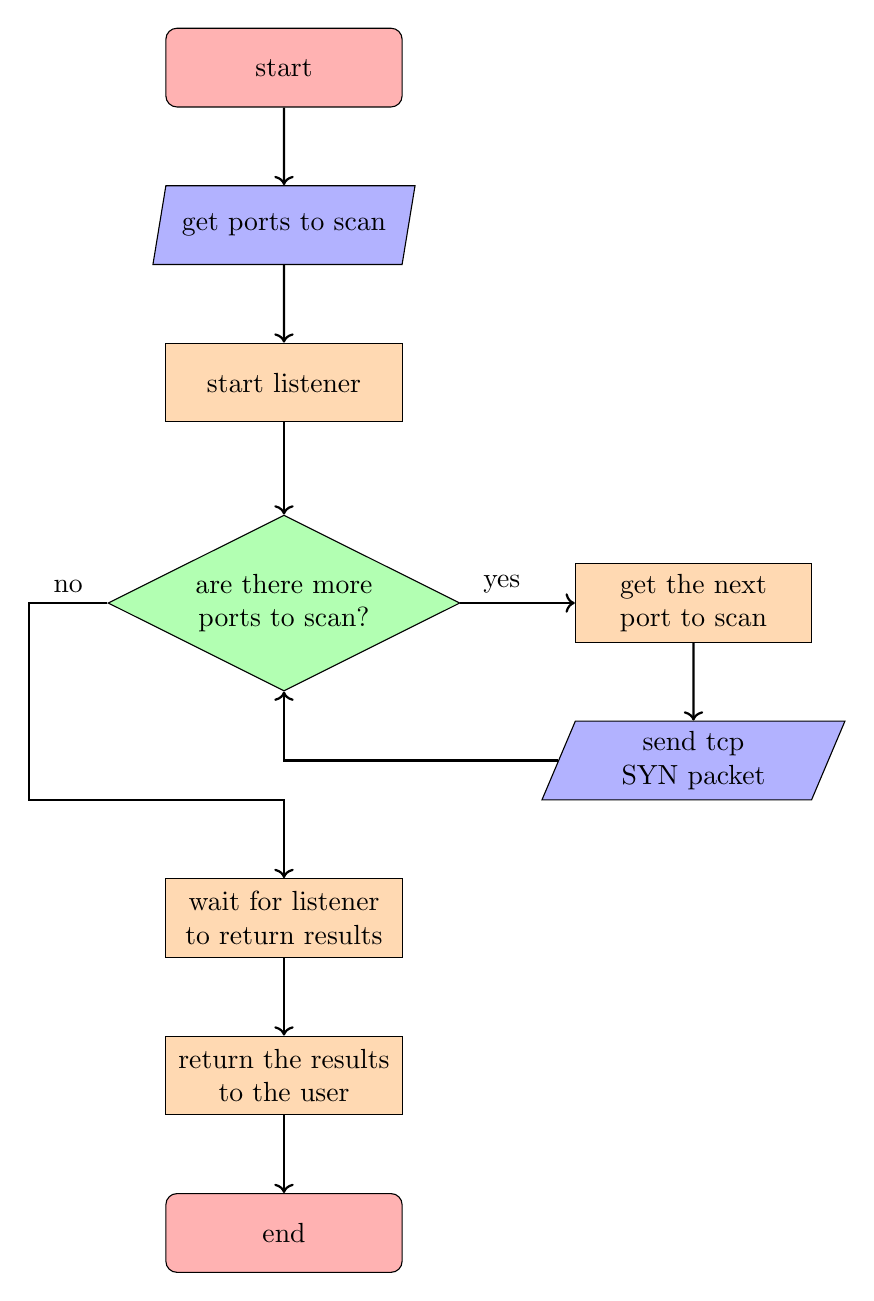
\begin{tikzpicture}[node distance=2cm]
      \node [startstop] (start) {start};
      \node [io, below of=start, text width=3cm] (input) {get ports to scan};
      \node [process, below of=input] (listener) {start listener};
      \node [decision, below of=listener, text width=3cm, yshift=-0.8cm] (loop) {are there more ports to scan?};
      \node [process, right of=loop, xshift=3.2cm] (get) {get the next port to scan};
      \node [io, below of=get, text width=3cm] (send) {send \gls{tcp} SYN packet};
      \node [process, below of=loop, yshift=-2cm] (wait) {wait for listener to return results};
      \node [process, below of=wait] (output) {return the results to the user};
      \node [startstop, below of=output] (end) {end};

      \draw [arrow] (start) -- (input);
      \draw [arrow] (input) -- (listener);
      \draw [arrow] (listener) -- (loop);
      \draw [arrow] (loop) -- node[midway,above,xshift=-0.2cm] {yes} (get);
      \draw [arrow] (get) -- (send);
      \draw [arrow] (send) -| node[midway,above,xshift=2cm] {} (loop);
      \draw [arrow] (loop) -- ([xshift=-1cm]loop.west) node[above,xshift=0.5cm] {no} -- ([xshift=-1cm,yshift=-2.5cm]loop.west) -| (wait);
      \draw [arrow] (wait) -- (output);
      \draw [arrow] (output) -- (end);

    \end{tikzpicture}
  \end{framed}
  \caption{\textit{%
    The logic for how I will do TCP SYN scanning.
}}\label{tcpsynscanflow}
\end{figure}

\begin{figure}[H]
  \centering
  \begin{framed}
    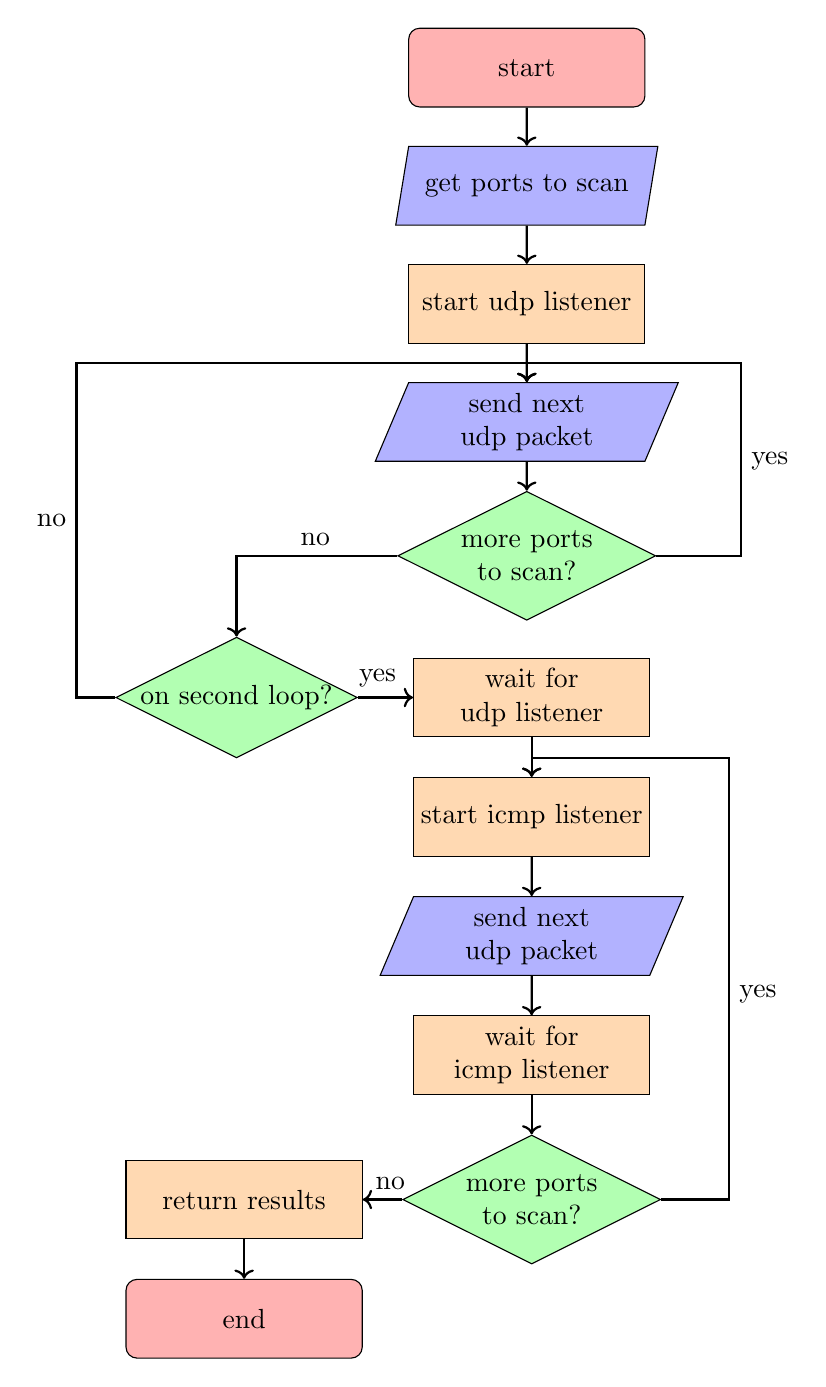
\begin{tikzpicture}[node distance=1.5cm]
      \node [startstop] (start) {start};
      \node [io,below of=start] (get) {get ports to scan};
      \node [process, below of=get] (udp listener) {start udp listener};
      \node [io, below of=udp listener, inner sep=0] (send 1) {send next \gls{udp} packet};
      \node [decision, below of=send 1, text width=2cm, yshift=-0.2cm] (loop 1) {more ports to scan?};
      \node [decision, below of=loop 1, left=0.5cm of loop 1, yshift=-0.3cm] (loop 2) {on second loop?};
      \node [process, right=0.7cm of loop 2] (udp wait) {wait for \gls{udp} listener};
      \node [process, below=0.5cm of udp wait] (icmp listener) {start \gls{icmp} listener};
      \node [io, below=0.5cm of icmp listener, inner sep=0] (send 2) {send next \gls{udp} packet};
      \node [process, below=0.5cm of send 2] (icmp wait) {wait for \gls{icmp} listener};
      \node [decision, below=0.5cm of icmp wait, text width = 2cm] (loop 3) {more ports to scan?};
      \node [process, left=0.5cm of loop 3] (return) {return results};
      \node [startstop, below=0.5cm of return] (end) {end};

      \draw [arrow] (start) -- (get);
      \draw [arrow] (get) -- (udp listener);
      \draw [arrow] (udp listener) -- (send 1);
      \draw [arrow] (send 1) -- (loop 1);
      \draw [arrow] (loop 1.east) -| ([xshift=1cm,yshift=0.75cm]send 1.east) node [right,yshift=-1.25cm] {yes} -| (send 1.north);
      \draw [arrow] (loop 1) -| node [above, xshift=1cm] {no} (loop 2);
      \draw [arrow] (loop 2.west) -| ([xshift=-4cm,yshift=0.75cm]send 1.west) node [left,yshift=-2cm] {no} -| (send 1.north);
      \draw [arrow] (loop 2) -- node [xshift=-0.1cm,above] {yes} (udp wait);
      \draw [arrow] (udp wait) -- (icmp listener);
      \draw [arrow] (icmp listener) -- (send 2);
      \draw [arrow] (send 2) -- (icmp wait);
      \draw [arrow] (icmp wait) -- (loop 3);
      \draw [arrow] (loop 3.east) -| ([xshift=1cm,yshift=0.75cm]icmp listener.east) node [right,yshift=-3cm] {yes} -| (icmp listener);
      \draw [arrow] (loop 3) -- node [above,xshift=0.1cm] {no} (return);
      \draw [arrow] (return) -- (end);

    \end{tikzpicture}
  \end{framed}
  \caption{\textit{%
    The logic behind how \gls{udp} scanning works.
}}\label{udpscanflow}
\end{figure}


\begin{figure}[H]
  \centering
  \begin{framed}
    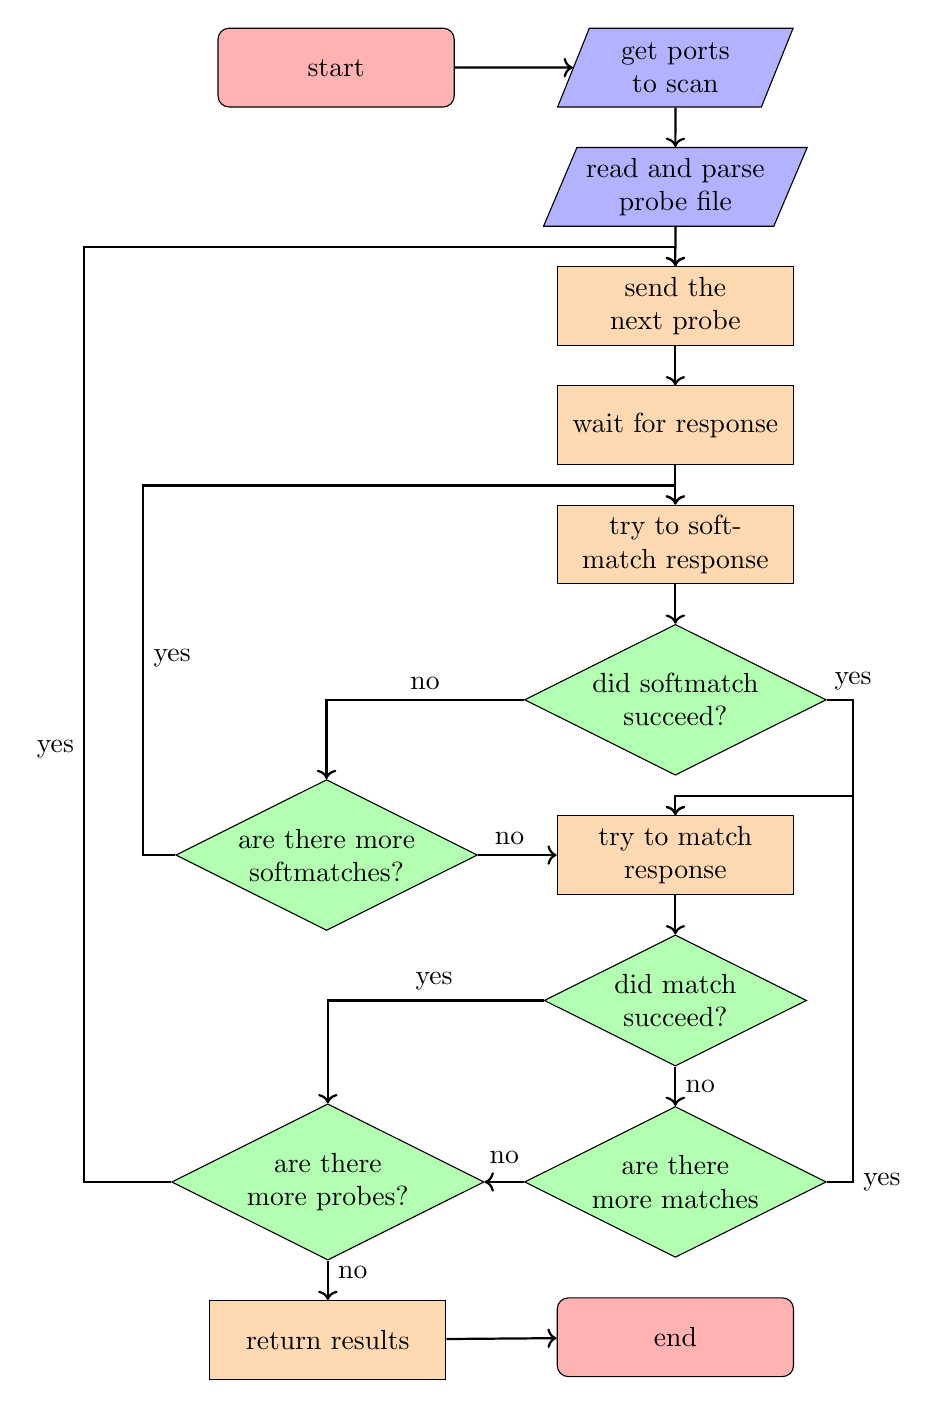
\begin{tikzpicture}[node distance=1.5cm]
      \node [startstop] (start) {start};
      \node [io, right=1.5cm of start, text width=2cm] (get ports) {get ports to scan};
      \node [io, below=0.5cm of get ports, text width=2.5cm] (parse probes) {read and parse probe file};
      \node [process, below=0.5cm of parse probes] (send probe) {send the next probe};
      \node [process, below=0.5cm of send probe] (wait) {wait for response};
      \node [process, below=0.5cm of wait] (softmatch) {try to softmatch response};
      \node [decision, below=0.5cm of softmatch, text width=2.5cm] (softmatched) {did softmatch succeed?};
      \node [process, below=0.5cm of softmatched] (match) {try to match response};
      \node [decision, left=1cm of match, text width=2.5cm] (softmatch loop) {are there more softmatches?};
      \node [decision, below=0.5cm of match, text width=2cm] (matched) {did match succeed?};
      \node [decision, below=0.5cm of matched, text width=2.5cm] (match loop) {are there more matches};
      \node [decision, left=0.5cm of match loop, text width=2.5cm] (probe loop) {are there more probes?};
      \node [process, below=0.5cm of probe loop] (return) {return results};
      \node [startstop, below=0.5cm of match loop] (end) {end};

      \draw [arrow] (start) -- (get ports);
      \draw [arrow] (get ports) -- (parse probes);
      \draw [arrow] (parse probes) -- (send probe);
      \draw [arrow] (send probe) -- (wait);
      \draw [arrow] (wait) -- (softmatch);
      \draw [arrow] (softmatch) -- (softmatched);
      \draw [arrow] (softmatched.east) -| node[above] {yes} ([yshift=0.75cm,xshift=0.75cm]match.east) -| (match);
      \draw [arrow] (softmatched) -| node[above, xshift=1.25cm] {no} (softmatch loop);
      \draw [arrow] (softmatch loop) -- node [above, xshift=-0.1cm] {no} (match);
      \draw [arrow] (softmatch loop)-|node[right,yshift=2.5cm]{yes}([xshift=-5.25cm,yshift=0.75cm]softmatch.west)-|(softmatch);
      \draw [arrow] (match) -- (matched);
      \draw [arrow] (match loop) -| node [right,] {yes} ([xshift=0.75cm,yshift=0.75cm] match.east) -| (match.north);
      \draw [arrow] (matched) -- node [right] {no} (match loop);
      \draw [arrow] (match loop) -- node [above, yshift=0.1cm] {no} (probe loop);
      \draw [arrow] (matched) -| node [above, xshift=1.35cm] {yes} (probe loop);
      \draw [arrow] (probe loop) -| node [left,yshift=5.5cm] {yes} ([xshift=-6cm,yshift=0.75cm]send probe.west) -| (send probe);
      \draw [arrow] (probe loop) -- node [midway, right, yshift=0.1cm] {no} (return);
      \draw [arrow] (return) -- (end);

    \end{tikzpicture}
  \end{framed}
  \caption{\textit{%
    The logic behind how version detection works.
}}\label{versiondetectflow}
\end{figure}


\subsection{Input data validation}

I plan to perform data validation in all of the functions in the fundamental modules
which will hold the basic functionality for my project, such as the scanning functions.
This is because my project will revolve heavily around these functions and they
will need to be as error free as possible.
Adding input validation to these core functions will enable me to find
errors in my code earlier.
For example, passing a function a list of strings instead of just a string might work in some cases,
but the function will have a completely different result.
These types of programming errors can be quite hard to debug,
as although they may not generate errors very often but on occasions they will still break the application.
Although data validation helps when programming, it will mainly be there to guide the user by showing them where
in their arguments the problem is. This is far more useful than some programs, which simply exit with
no information, beyond the fact that error occurred.

An example for a Python ValueError could be trying to turn the string \\
\verb|"tacos"|
into an integer. This will result in the following error message:\\
\verb|ValueError: invalid literal for int() with base 10: `tacos'| \\
This informs you that you have tried to turn \verb|"tacos"|
into an integer with base 10, which is invalid.
This is a clear and helpful error message,
because it tells you what you tried to do that went wrong,
and which argument was the one that caused the error.

\subsection{Algorithm for complex structures}

\begin{algorithm}
  \caption{\textit{%
  My algorithm for turning a \gls{cidr}-specified \gls{subnet} into a list of actual \gls{ipaddr}es
}}\label{ip_range}
  \begin{algorithmic}[1]
    \Procedure{ip\_range}{}
    \State{$\textit{network\_bits} \gets \text{number of network bits specified}$}
    \State{$\textit{ip} \gets \text{base IP address}$}
    \State{$\textit{mask} \gets 0$}
    \For{$\textit{maskbit} \gets (32-\textit{network\_bits}),31$}
      \State{$\textit{mask} \gets \textit{mask} + 2^\textit{maskbit}$}
    \EndFor{}
    \State{$\textit{lower\_bound} \gets \text{\textit{ip} AND \textit{mask}}$}
    \Comment{zero the last 32-\textit{network\_bits}}
    \State{$\textit{upper\_bound} \gets \text{\textit{ip} OR (\textit{mask} XOR 0xFFFFFFFF)}$}
    \Comment{turn the last 32-\textit{network\_bits} to ones}
    \State{$\textit{addresses} \gets \text{empty list}$}
    \For{$\textit{address} \gets \textit{lower\_bound},\textit{upper\_bound}$}
      \State{append \Call{convert\_to\_dot}{\textit{address}} to \textit{addresses}}
    \EndFor{}
    \Return{\textit{addresses}}
    \EndProcedure{}
  \end{algorithmic}
\end{algorithm}

\begin{algorithm}
  \caption{\textit{%
    My algorithm for pretty-printing a dictionary of lists of\gls{port}numbers
    such that ranges are specified as start-end instead of start,start+1,\ldots,end
}}\label{collapse}
  \begin{algorithmic}[1]
  \Procedure{collapse}{}
    \State{$\textit{port\_dictionary} \gets \text{dictionary of lists of\gls{port}numbers}$}
    \State{$\textit{key\_results} \gets \text{empty list}$}
    \Comment{stores the formatted result for each key}
    \For{\textit{key} in \textit{port\_dictionary}}
      \State{$\textit{ports} \gets \text{\textit{port\_dict}[\textit{key}]}$}
      \State{$\textit{result} \gets \textit{key} + \text{``:\{''}$}
      \If{\textit{ports} is empty}
        \State{$\textit{new\_sequence} \gets FALSE$}
        \For{$\textit{index} \gets 1,\text{(length of \textit{ports})}-1$}
          \State{$\textit{port} = \text{\textit{ports}[\textit{index}]}$}
          \If{$\textit{index} = 0$}
            \State{$\textit{result} \gets \textit{result} + \textit{ports}[0]$}
            \Comment{append the first element}
            \If{$\text{\textit{ports}[\textit{index}+1]} = \textit{port} + 1$}
              \State{$\textit{result} \gets \textit{result}+\text{``-''}$}
              \Comment{begin a new sequence}
            \Else{}
              \State{$\textit{result} \gets \textit{result} + \text{``,''}$}
              \Comment{not a sequence}
            \EndIf{}
          \ElsIf{$\textit{port} + 1 \not= \text{\textit{ports}[\textit{index}+1]}$}
          \Comment{break in sequence}
            \State{$\textit{result} \gets \textit{result} + \textit{port} + \text{``,''}$}
            \State{$\textit{new\_sequence} \gets \textit{TRUE}$}
          \ElsIf{$\textit{port}+1 = \text{\textit{ports}[\textit{index}+1]} \And \textit{new\_sequence}$}
            \State{$\textit{result} \gets \textit{result} + \text{``-''}$}
            \State{$\textit{new\_sequence} \gets \textit{FALSE}$}
          \EndIf{}
        \EndFor{}
      \State{$\textit{result} \gets \textit{result} + \text{\textit{ports}[(length of \textit{ports})-1]} + \text{``\}''}$}
      \State{append \textit{result} to \textit{key\_results}}
      \EndIf{}
    \EndFor{}
    \Return{``\{'' + (\textit{key\_results} separated by ``, '') + ``\}''}
  \EndProcedure{}
  \end{algorithmic}
\end{algorithm}

\section{Technical Solution}
I have placed all of my code in Appendix~\ref{code}. 
I will be going through each of the items in this appendix and explaining what they do.

Appendix~\ref{app:icmpping} contains all the code which I wrote while in an early experimentation
phase where I was testing out how I was planning to make and structure the project.

Appendix~\ref{app:pingscanner} contains all the code which I wrote while writing the initial prototype
of my ping scanner which uses \gls{icmp} \verb|echo request| messages to detect hosts which are online on a given
subnet.
This is used to meet success criterion~\ref{ping}.

Appendix~\ref{app:subnettoaddresses} contains all the code which I wrote while writing a tool to
translate a \gls{cidr}-specified subnet into the list of \gls{ip} addresses for that subnet.
It uses logic to exclude the broadcast address and host addresses for each subnet.
This is used to meet success criterion~\ref{cidr}.

Appendix~\ref{app:tcpscan} contains all of the prototypes for \gls{tcp}-based scanning,
which are contained in the sub-appendices~\ref{app:connectscan} and~\ref{app:synscan}.
Appendix~\ref{app:connectscan} contains all of the code which I created whilst prototyping connect scanning.
It satisfies success criteria~\ref{tcpopen} and~\ref{tcpclosed}.
Appendix~\ref{app:synscan} contains all of the code I wrote while prototyping \gls{tcp} SYN scanning.
It satisfies success criteria~\ref{tcpopen},~\ref{tcpclosed} and~\ref{tcpfiltered}.

Appendix~\ref{app:udpscan} contains all of the code I wrote while prototyping \gls{udp} scanning.
It satisfies success criteria~\ref{udpopen},~\ref{udpclosed} and~\ref{udpfiltered}.

Appendix~\ref{app:versiondetection} contains all of the code I wrote while prototyping version detection
scanning. It satisfies success criteria~\ref{servicedetect} and~\ref{versiondetect}.

Appendix~\ref{app:modules} contains all of the modules I wrote to help with creating my main application,
described later.
These modules mainly contain code which I reuse often,
such as code to calculate an ip checksum, or validate an \gls{ipaddr}.

Appendix~\ref{app:examples} contains a script I wrote which will run each of the prototype applications I made.
This doesn't satisfy any of the success criteria,
but was very useful for solving issues I had with importing Python modules,
where owing to the directory structure everything has to be started from the root of the directory structure,
otherwise errors occur.
My solution for eliminating the errors was to run everything at the root of the directory structure,
as this can call the \verb|main()| function defined in each of the modules,
and can also import all of the modules in the modules directory.

Appendix~\ref{app:netscan} contains the code for my final application.
This satisfies all of the success criteria apart from~\ref{osdetect},
which as previously discussed, is alternatively completed via version detection scanning.

Appendix~\ref{app:tests} contains all of the code for my unit tests which I run using \\
\verb|Python -m pytest|.
It automatically runs each function, and delivers verbose information on each one.
I have deliberately named all of the test functions in a very verbose way and I only test one thing in each function.
This means that it is much easier for me to read from the name of a failed test exactly what went wrong
with what function and what argument caused it.
An example of this can be seen in Figure~\ref{testing},
where I have changed one of the tests so that it fails.
You can see that the output of the test shows me a clear difference between what
was expected on one side of the assertion statement
and then what actually happened on the other side.
In this case,
it shows that in the left set there is an extra element ``192.168.1.1''
and in the right an extra element ``192.168.1.0''.
This is very helpful for preventing regressions in the code.
Until I wrote these unit tests,
I found that I would write a new feature and accidentally break
another piece of functionality as a consequence.

\begin{figure}[H]
  \centering
  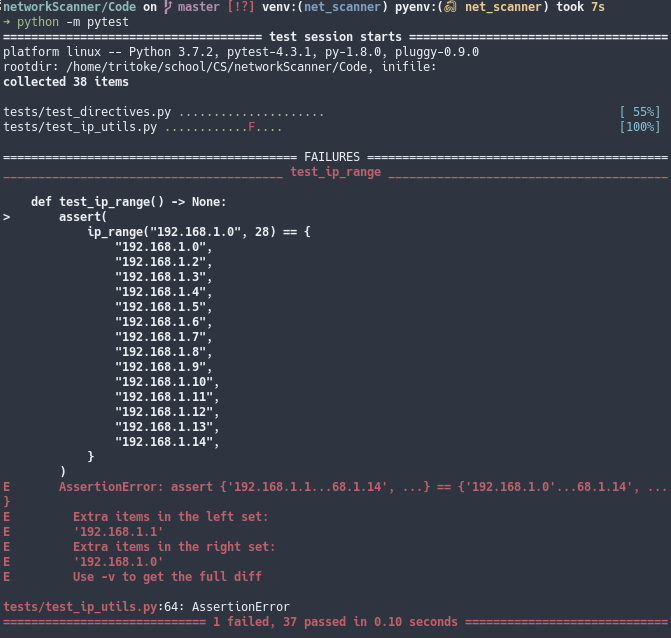
\includegraphics[width=\textwidth]{testing.png}
  \caption{\textit{%
    A screenshot of running pytest with a deliberately broken test.
}}\label{testing}
\end{figure}

\section{Testing}

\subsection{Test Plan}

I will be testing my application using a combination of unit tests,
and Wireshark where applicable.
Unit tests are more suitable for doing tests on specific functions to make sure
that regressions don't occur while developing the application.
A regression is a when a feature or change that was implemented into the program 
has accidental consequences that cause the application to break.
I will use Wireshark to show the scanning portion of my code,
and when external connections are made/custom packets created.
Section~\ref{wiresharktests} contains the tests using Wireshark;
the unit tests are in Appendix~\ref{app:tests}.

The Wireshark testing will require Wireshark and iptables.
I will need to set up Wireshark in listen mode on the right interface so that it
captures the packets that my program is sending.
From there I will be able to inspect the sent packets and determine whether they fit
what was expected in the test description or whether they don't match at all.
For filtered packet tests I will need to run the command \verb|iptables -I INPUT -s 127.0.0.1 -j DROP|
and scan the localhost address, and after the test I will need to run the command \verb|iptables -F| 
to flush all the iptables rules to prevent any confusion in future caused by an firewall rule
that shouldn't be there.

To running the unit tests will require Python 3.7.2 and pytest 4.3.1.
To run the tests I will need to run \verb|python -m pytest| inside the Code directory.
This will call pytest,
which will find the tests inside the tests directory and run them.
It will then display the number of tests that passed along with lots of information on the
tests that failed, such as what the arguments were etc.
Pytest does this via introspection of the comparison and assert commands.
This means that it uses its own versions of those commands which allow it to get more
information out about what went wrong,
such as which element in a list was the one that caused the comparison to return false etc.

\subsection{Testing Evidence}\label{wiresharktests}

\subsubsection{Printing a usage message when run without parameters}

To show this I will run my program passing it no parameters.
This should print out a message of the form: \verb|USAGE: ./<program> <required> <parameters>|
where everything in angle brackets should be replaced by what is necessary for my program. 
In Figure~\ref{noparametertest} you can see me run \verb|./netscan.py| with no parameters and it
prints out the required usage message telling me that I am missing the target\_spec parameter, this
shows that it passed this test.
This shows success criterion~\ref{usage}.
\begin{figure}[H]
  \centering
  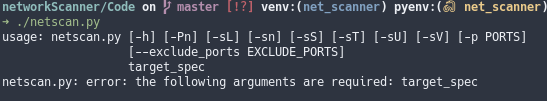
\includegraphics[width=\textwidth]{noparameters.png}
  \caption{\textit{%
    Screenshot showing my program being run without parameters.
}}\label{noparametertest}
\end{figure}

\subsubsection{Printing a help message when passed -h}

To show this I will run my program with the \verb|-h| flag.
This should print out a message showing each of the options as well as what each of them do.
It should also print out whether they are positional arguments or optional arguments and if
an argument can have two forms then it should print out both forms of the flag, i.e. \verb|-p --ports|.
In Figure~\ref{hflagtest} you can see me run my program with the \verb|-h| flag and it proceeds to
print of a help message with messages with what each option is for as well as short and long form of
arguments, this shows my program passed this test.
This shows success criterion~\ref{usage}.

\begin{figure}[H]
  \centering
  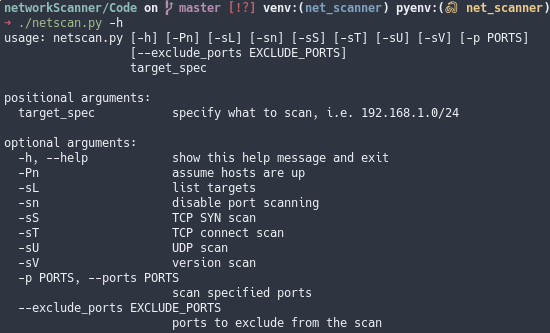
\includegraphics[width=\textwidth]{hmessage.png}
  \caption{\textit{%
    Screenshot showing my program being run with the -h flag.
}}\label{hflagtest}
\end{figure}

\subsubsection{Printing a help message when passed -help}
To show this I will run my program with the \verb|--help| flag.
This should produce the same output as with \verb|-h|.
This shows the same message as in the test of \verb|-h|.
To prove this,
if I take the sha1sum of the output for both flags,
we can see that the hashes are identical and therefore the originals were also identical;
this is shown in Figure~\ref{messagehash}.
This shows success criterion~\ref{usage}.

\begin{figure}[H]
  \centering
  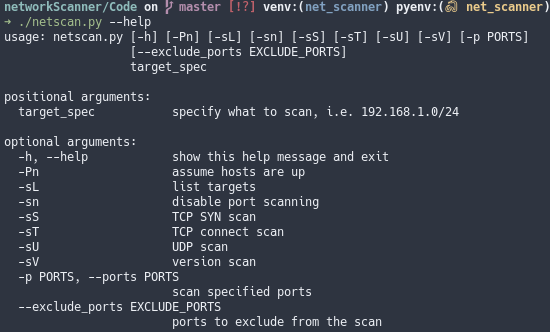
\includegraphics[width=\textwidth]{helpmessage.png}
  \caption{\textit{%
    Screenshot showing my program being run with the help flag.
}}\label{helpflagtest}
\end{figure}

\begin{figure}[H]
  \centering
  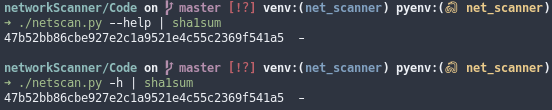
\includegraphics[width=\textwidth]{messagehashes.png}
  \caption{\textit{%
    Screenshot showing the hashes of the two help messages.
}}\label{messagehash}
\end{figure}

\subsubsection{Scanning a subnet with ICMP echo request messages}
To show this I will run my program with the \verb|-sn| flag and specify the
subnet of my local network \verb|192.168.178.0/24|.
This should produce a list of all the hosts which are up on the network.
In Figure~\ref{lanscantest} you can see you can see my program's output
showing that the hosts:
\begin{itemize}
  \item{192.168.178.60}
  \item{192.168.178.56}
  \item{192.168.178.30}
  \item{192.168.178.1}
\end{itemize}
all responded with \gls{icmp} echo reply messages.
This is reflected in a packet capture I took while performing the scan.
A section of this scan is shown in Figure~\ref{lanscanWireshark},
where you can see some of \gls{icmp} echo request messages my program sent,
along with some of the requests to hosts that don't exist.
Note the different addresses in the source and destination fields,
and the Echo (ping) request vs reply in the info column.
This meets success criteria~\ref{blackbox} and~\ref{ping}.

\begin{figure}[H]
  \centering
  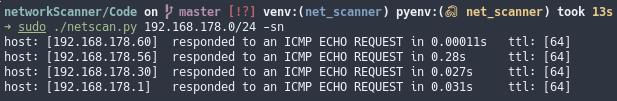
\includegraphics[width=\textwidth]{pingscantest.png}
  \caption{\textit{%
    Screenshot showing the output of a scan of my local network.
}}\label{lanscantest}
\end{figure}

\begin{figure}[H]
  \centering
  \includegraphics[width=\textwidth]{pingscantest_Wireshark.png}
  \caption{\textit{%
    Screenshot showing a selection of the packets being sent by this scan.
}}\label{lanscanWireshark}
\end{figure}

\subsubsection{Translating a CIDR-specified subnet into a list of IP addresses}
To show this I will run my program with the \verb|-sL| flag and I will specify
a small subnet of \verb|192.168.1.0/28| (I have chosen such a small subnet
such that it will fit on my terminal and therefore in a screenshot).
I expect the list of addresses to be \verb|192.168.1.1 - 192.168.1.14|.
To prove that my program works,
I will screenshot the output when run with the stated parameters and I will use
a website to translate the same subnet and show
that it displays the same addresses as my program.
In Figure~\ref{cidrtest}, you can see that the output from my program matches
the expected list of IP addresses from \verb|192.168.1.1| to \verb|192.168.1.14|
which is also shown by the screen shot of the same subnet translated by
the ipcalc utility on Linux.
This proves my program works and covers success criterion~\ref{cidr}.

\begin{figure}[H]
  \centering
  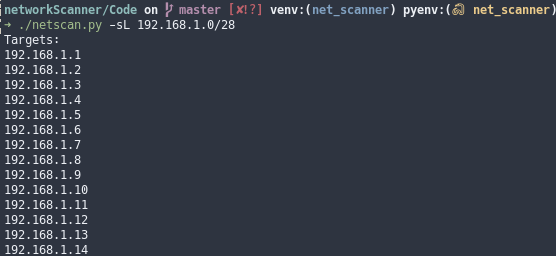
\includegraphics[width=\textwidth]{iplist.png}
  \caption{\textit{%
    Screenshot showing the output of my program when asked to translate the subnet 192.168.1.0/28.
}}\label{cidrtest}
\end{figure}

\begin{figure}[H]
  \centering
  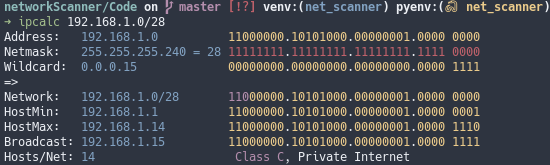
\includegraphics[width=\textwidth]{ipcalclist.png}
  \caption{\textit{%
    Screenshot showing the range displayed by the ipcalc utility when asked to calculate
    the same subnet.
}}\label{cidrwebproof}
\end{figure}

\subsubsection{Scanning without first checking whether hosts are up.}
To show this I will perform a TCP scan on a small subnet where I
know there are no hosts and show that the scan continues despite there actually
being no host on the other end. To do this I will pass the \verb|-Pn| flag
and I will specify the subnet \verb|192.168.43.0/28| which I know has no has no hosts
on it. I will also specify \verb|-p 12345| to only scan port 12345 so that there are
fewer requests in the packet capture. Finally I will specify \verb|-sS| to do \gls{tcp}
SYN SCANNING.\@ I expect to see a multiple of 14 \gls{arp} messages.
This is because I don't know how many times my \gls{nic} will retry at getting
the destination \gls{mac} address. It needs the destination \gls{mac} address to send
the packet to its destination as we are scanning a private IP range of my router.
In Figure~\ref{nocheckoutput} you can see the output of my program when run with the
specified flags, you can see that as expected it showed that there were no open ports
on those machines as they don't exist. In Figure~\ref{nocheckWireshark} you can see the
packet capture of the packets my code sent, however, there are only ARP messages, this is
because we are scanning in the private IP range of my router which was the only
way I could guarantee that there was no machine at the other end. However, this is
as expected, as well as this we can see 42 \gls{arp} requests, which is $3\times14$
\gls{arp} requests, which would indicate each scan made three \gls{arp} requests before
giving up. This shows my program can perform scans without first checking if the host is
up, showing success criterion~\ref{nocheck}.
\begin{figure}[H]
  \centering
  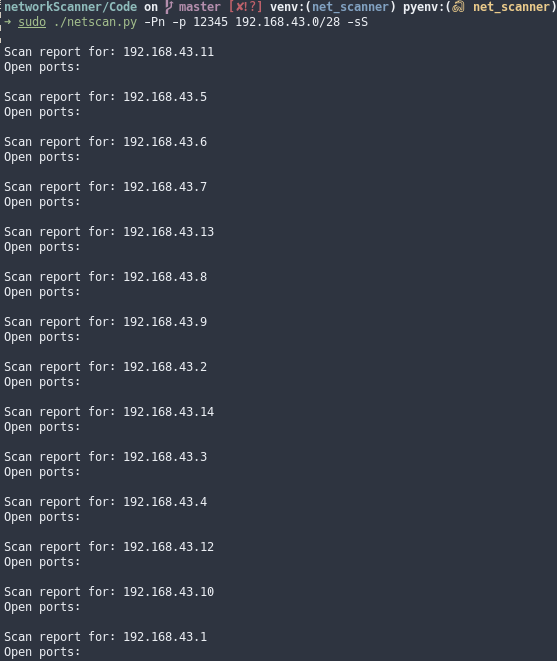
\includegraphics[width=\textwidth]{nocheckhostoutput.png}
  \caption{\textit{%
    Screenshot showing the output from my code when asked to port scan a subnet
    with no machines behind the addresses.
}}\label{nocheckoutput}
\end{figure}

\begin{figure}[H]
  \centering
  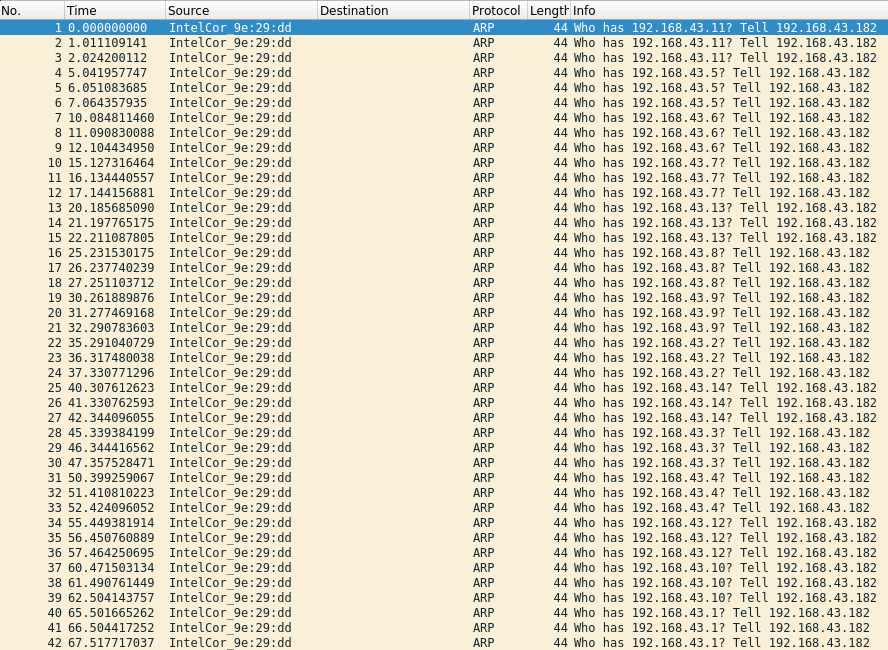
\includegraphics[width=\textwidth]{nocheckpcap.png}
  \caption{\textit{%
    Screenshot showing the ARP requests my NIC sent to attempt to determine
    where to send the attempted connection packets.
}}\label{nocheckWireshark}
\end{figure}

\subsubsection{Detecting whether a TCP port is open}
To show this I will perform a \gls{tcp} \verb|Connect()| scan on my local
machine while running a script which will listen on port 12345 for any connections
and send back a message. I will pass my program the flags \verb|-sT| and
\verb|-p 12345| as well as specifying localhost to scan (127.0.0.1).
I expect to see a \gls{tcp} SYN-ACK handshake between my program and the script and
then my program to output that the port is open. In Figure~\ref{tcpopenpcap} you can
see the expected \gls{tcp} SYN-ACK handshake performed by my program and the script
in Figure~\ref{tcpopenscript}.
You can see the output of my program in Figure~\ref{tcpopenoutput}; as expected
it outputs that port 12345 is open. This shows success criteria~\ref{blackbox}
and~\ref{tcpopen}.

\begin{figure}[H]
  \centering
  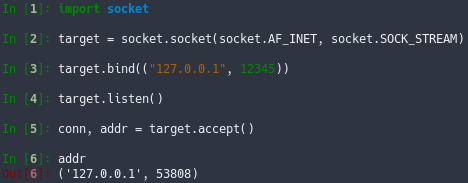
\includegraphics[width=\textwidth]{tcpopenscript.png}
  \caption{\textit{%
    Screenshot showing the script I ran to accept a connection on localhost port 12345.
}}\label{tcpopenscript}
\end{figure}

\begin{figure}[H]
  \centering
  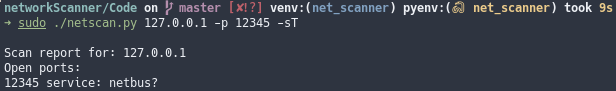
\includegraphics[width=\textwidth]{tcpopenoutput.png}
  \caption{\textit{%
    Screenshot showing the output of my script when run with the specified flags
    and while the script in Figure~\ref{tcpopenscript} was running.
}}\label{tcpopenoutput}
\end{figure}

\begin{figure}[H]
  \centering
  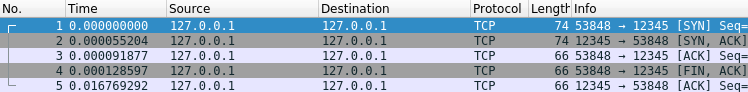
\includegraphics[width=\textwidth]{tcpopenpcap.png}
  \caption{\textit{%
    Screenshot showing the packet capture of the TCP SYN-ACK handshake performed
    by the scan in Figure~\ref{tcpopenoutput} with the script in~\ref{tcpopenscript}.
}}\label{tcpopenpcap}
\end{figure}

\subsubsection{Detecting whether a TCP port is closed}
To show this, I will perform a \gls{tcp} \verb|Connect()| scan
on my local machine, except that instead of running a script to catch the
request, I will just let it try to connect to the closed port.
I expect to see a \gls{tcp} SYN packet sent to the port, and then a RST ACK
packet sent back; my program should output no open ports.
I will pass my program the same options as in the test for
a \gls{tcp} open port.
In Figure~\ref{tcpclosedpcap}, you can see the attempted connection to
127.0.0.1 port 12345, along with the RST ACK packet afterwards, indicating
the port is closed. This is reflected in Figure~\ref{tcpclosedoutput}
with no open ports, showing success criteria~\ref{blackbox} and~\ref{tcpclosed}.
\begin{figure}[H]
  \centering
  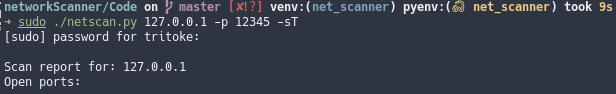
\includegraphics[width=\textwidth]{tcpclosedoutput.png}
  \caption{\textit{%
    Screenshot showing the output of my program when run with the specified options.
}}\label{tcpclosedoutput}
\end{figure}

\begin{figure}[H]
  \centering
  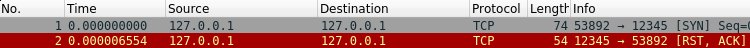
\includegraphics[width=\textwidth]{tcpclosedpcap.png}
  \caption{\textit{%
    Screenshot showing the packet capture of the TCP SYN-RST closed port indication
    caused by the scan in Figure~\ref{tcpclosedoutput}.
}}\label{tcpclosedpcap}
\end{figure}

\subsubsection{Detecting whether a TCP port is filtered}
To show this I will perform a \gls{tcp} SYN scan on localhost port 12345,
except that I will also introduce a firewall rule to drop all requests to localhost.
I expect this to produce no response to the initial SYN packet sent by my
program, and my program to output that port as filtered. To test this, I will
run my program with the flags \verb|-sS,-p 12345,-Pn|. 
This will instruct it to perform a TCP SYN scan on port 12345 and not to check that the
host is up before beginning the scan.
I will also introduce a firewall rule using the Linux iptables utility to drop
all requests to localhost as so: \verb|iptables -I INPUT -s 127.0.0.1 -j DROP|.
The output of my program is shown in Figure~\ref{tcpfilteredoutput}.
It can be seen that port 12345 is displayed as filtered, and in the packet capture shown in
Figure~\ref{tcpfilteredpcap}, you can see that there is no response to our initial packet,
which corresponds to what I thought would happen with an iptables rule in place
to drop packets. This shows success criteria~\ref{blackbox} and~\ref{tcpfiltered}.

\begin{figure}[H]
  \centering
  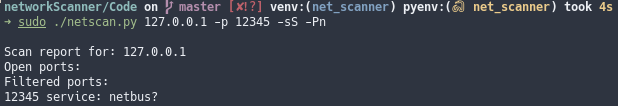
\includegraphics[width=\textwidth]{tcpfilteredoutput.png}
  \caption{\textit{%
    Screenshot showing the output of my program when run with the specified options
    and a firewall in place to drop all packets to 127.0.0.1.
}}\label{tcpfilteredoutput}
\end{figure}

\begin{figure}[H]
  \centering
  
\includegraphics[width=\textwidth]{tcpfilteredpcap.png}
  \caption{\textit{%
    Screenshot showing the packet capture of the scan in Figure~\ref{tcpfilteredoutput}
}}\label{tcpfilteredpcap}
\end{figure}

\subsubsection{Detecting whether a UDP port is open}
To show this I will perform a \gls{udp} scan on a script I had already written while
developing \gls{udp} scanning.
This can be seen in Listing~\ref{udpopenscript}.
I expect to see my program output port 12345 as open, and in the packet capture, I
expect to see two \gls{udp} packets followed by two response \gls{udp} packets from my
listener program. I will test this using the following flags: \verb|-Pn,-p 12345,-sU|.
These translate to scanning port 12345 over UDP and not checking the host is up beforehand.
In Figure~\ref{udpopenoutput}, you can see the output of my program when run as specified,
and you can see that it correctly detects port 12345 as being open.
In Figure~\ref{udpopenpcap}, you can see the packet capture of my program being run.
However, the output was not precisely as expected,
as I did not foresee the \gls{icmp} destination unreachable messages,
which were sent by the kernel in response to the UDP probe.
However, apart from those messages,
the capture shows the program detecting the \gls{udp} port was open,
as expected. This meets success criteria~\ref{blackbox} and~\ref{udpopen}.

\lstinputlisting[firstline=3,caption=\textit{Script to open port 12345 to UDP.},label=udpopenscript]{../../Code/udp_scan/open_X_port_to_UDP.py}

\begin{figure}[H]
  \centering
  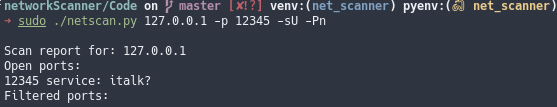
\includegraphics[width=\textwidth]{udpopenoutput.png}
  \caption{\textit{%
    Screenshot showing the output of my program when run with the options specified
    above, and the script in Listing~\ref{udpopenscript} is running.
}}\label{udpopenoutput}
\end{figure}

\begin{figure}[H]
  \centering
  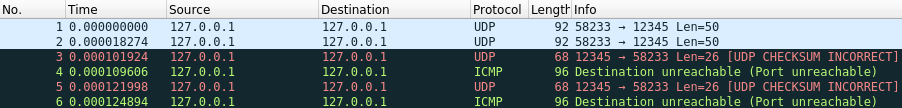
\includegraphics[width=\textwidth]{udpopenpcap.png}
  \caption{\textit{%
    screenshot showing the packet capture of the scan in Figure~\ref{udpopenoutput}
}}\label{udpopenpcap}
\end{figure}

\subsubsection{Detecting whether a UDP port is closed}
To show this I will perform a \gls{udp} scan on a port which
has no service listening behind it. I expect my program to print out
no filtered ports and no open ports, showing that the port was closed.
In the packet capture, I expect to see three \gls{udp} packets and three response
\gls{icmp} packets. To test this, I will use my program with the following flags:
\verb|-p 12345,-Pn,-sU| which perform a \gls{udp} port scan without first checking
if the host is up. In Figure~\ref{udpclosedoutput}, you can see the output of my program
when run with the options specified above.
There are no ports displayed as either open or filtered.
This shows that my program successfully identified the port as closed.
This shows success criteria~\ref{blackbox} and~\ref{udpclosed}.

\begin{figure}[H]
  \centering
  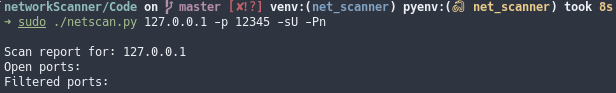
\includegraphics[width=\textwidth]{udpclosedoutput.png}
  \caption{\textit{%
    screenshot showing the output of my program when scanning with the
    options specified above.
}}\label{udpclosedoutput}
\end{figure}

\begin{figure}[H]
  \centering
  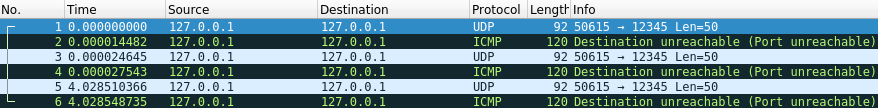
\includegraphics[width=\textwidth]{udpclosedpcap.png}
  \caption{\textit{%
    screenshot showing the packet capture of the scan in Figure~\ref{udpclosedoutput}
}}\label{udpclosedcap}
\end{figure}

\subsubsection{Detecting whether a UDP port is filtered}
To show this I will use my program to perform a \gls{udp} scan on my local machine
with a firewall rule to drop any ports sent to the localhost address. I expect to see
my program to output the port as filtered and in the packet capture I expect to see
three \gls{udp} packets with no response to any of them.
In Figure~\ref{udpfilteredoutput} you can see my program correctly identifies
the port as being filtered, and in Figure~\ref{udpfilteredpcap} you can see
the packet capture of the scan which also as expected shows the three \gls{udp}
packets with no reply packets. This shows the program meeting success criteria~\ref{blackbox}
and~\ref{udpfiltered}.

\begin{figure}[H]
  \centering
  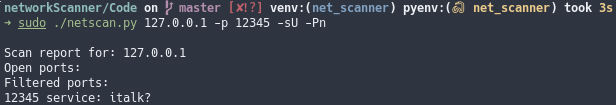
\includegraphics[width=\textwidth]{udpfilteredoutput.png}
  \caption{\textit{%
    screenshot showing the output of my program when scanning with the
    options specified above.
}}\label{udpfilteredoutput}
\end{figure}

\begin{figure}[H]
  \centering
  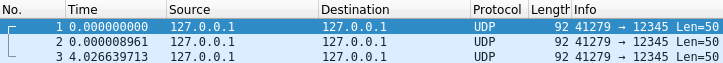
\includegraphics[width=\textwidth]{udpfilteredpcap.png}
  \caption{\textit{%
    screenshot showing the packet capture of the scan in Figure~\ref{udpfilteredoutput}
}}\label{udpfilteredpcap}
\end{figure}

\subsubsection{Detecting the operating system of another machine}
I haven't directly added this as a feature to my project, largely because
I discovered on implementing version scanning that this had the substantially the same effect.
I found that in most instances it was possible to detect an operating system-dependent
service and thereby deduce which operating system that machine was running.
For example, if a machine is open on \gls{tcp} port 22,
and \gls{ssh} is detected to be running behind that port,
then the machine is most likely running Linux, as \gls{rdp} is more commonly used
for this purpose on Windows machines.
It would become even more likely that the target machine runs Linux
if the scan reveals some further information such as the \gls{cpe}.
In Figure~\ref{sshversiondetect} you can see a scan of my machine where I have \gls{ssh} running.
My program reveals that the version is 7.9 and the vendor is openbsd, which is a Unix-like operating system.
This shows that my \gls{ssh} version is Unix-based and therefore that my machine is likely running Linux,
which is the case.
This partially completes success criterion~\ref{osdetect}.

\begin{figure}[H]
  \centering
  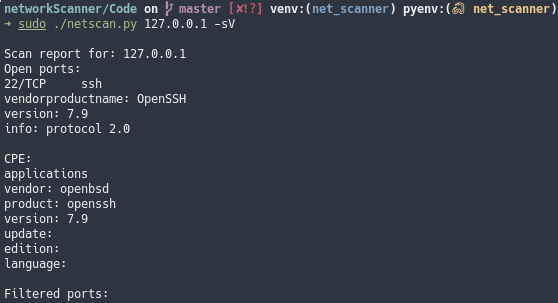
\includegraphics[width=\textwidth]{sshversiondetect.png}
  \caption{\textit{%
    screenshot showing a version scan of my local machine.
}}\label{sshversiondetect}
\end{figure}

\subsubsection{Detecting the service and its version running behind a port}
To show this I will use my program to perform a version detection scan on my local machine
while I am running \gls{ssh}. I expect to see my program identify that \gls{ssh} is running
on \gls{tcp} port 22 and that it detects it as OpenSSH version 7.9. To test this
I will run my program with the \verb|-sV| flag to indicate version detection and
I will run it against the localhost address. In Figure~\ref{versiondetect}
you can see that my program successfully identified \gls{ssh} as running on
\gls{tcp} port 22 as well as the expected identification of OpenSSH version 7.9
operating on protocol version 2.
It also identified some CPE information such as OpenSSH coming from the openbsd
distribution.
This meets success criteria~\ref{blackbox},~\ref{servicedetect} and~\ref{versiondetect}.

\begin{figure}[H]
  \centering
  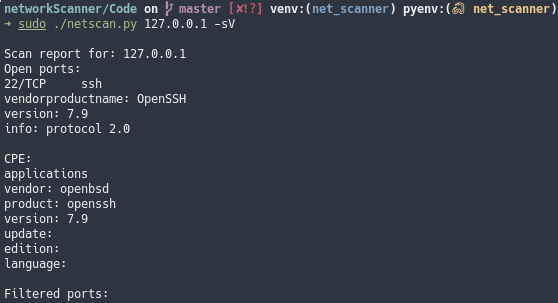
\includegraphics[width=\textwidth]{sshversiondetect.png}
  \caption{\textit{%
    screenshot showing a version scan of my local machine running ssh.
}}\label{versiondetecttest}
\end{figure}

\subsubsection{User enters invalid ip address}
To show this I will run my program with the \verb|target_spec|
option being \\
\verb|300.300.300.300| which is an invalid
IPv4 address, because each of the octets is not between 0 and 255.
I expect to see my program raise a Python ValueError
saying that this is an invalid dot form \gls{ipaddr},
and displaying \\
\verb|300.300.300.300| as the invalid \gls{ipaddr}.
In Figure~\ref{invalidip} you can see my program's output
for this invalid IP address. This shows a successful pass as it
correctly identifies the invalid IP and displays the error
and the argument that caused the error to the user.

\begin{figure}[H]
  \centering
  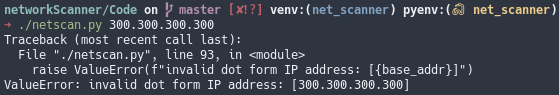
\includegraphics[width=\textwidth]{invalidip.png}
  \caption{\textit{%
    Screenshot showing the output from an invalid IP address being used.
}}\label{invalidip}
\end{figure}

\subsubsection{User enters invalid number of network bits}
To show this I will run my program and ask it to list the
\gls{ip} addresses specified by the subnet \verb|192.168.1.0/33|.
\gls{ip} addresses are only 32 bits, long so specifying 33
network bits has no meaning, and thus is invalid data.
I expect my program to raise a ValueError and print out
that it was an invalid number of network bits that caused
the error, along with 33 being the network bits.
In Figure~\ref{invalidnetworkbits} you can see that
my program successfully identified the invalid number of network bits,
raised the expected error, and printed the expected information.

\begin{figure}[H]
\centering
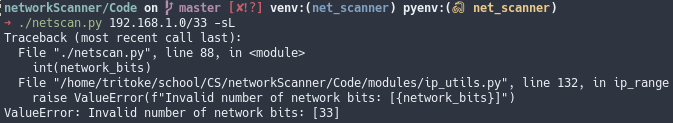
\includegraphics[width=\textwidth]{invalidnetworkbits.png}
\caption{\textit{%
  Screenshot showing the output of my program when passed
  an invalid number of network bits.
}}\label{invalidnetworkbits}
\end{figure}

\subsubsection{User enters an invalid port number to scan}
To show this I will run my program with the argument \verb|-p 99999|.
Because port numbers can only go up to 65535, this is erroneous data,
and as such should generate an error message specifying that 
you have tried to scan an invalid destination port.
In Figure~\ref{invalidportnum} you can see that my program
successfully identified 99999 as an invalid destination port
and printed the correct error message accordingly.

\begin{figure}[H]
\centering
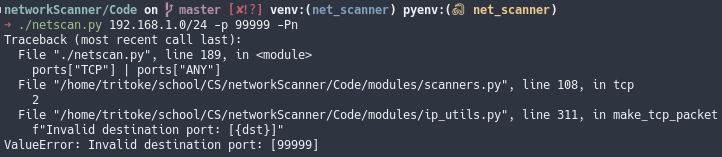
\includegraphics[width=\textwidth]{invalidportnum.png}
\caption{\textit{%
  Screenshot of my program showing the output from an invalid port number.
}}\label{invalidportnum}
\end{figure}

\subsubsection{User enters an invalid number of network bits and a bad IP address}
To show this I will run my program with both an invalid \gls{ipaddr} and an
invalid port number. I expect this to raise a ValueError for the invalid \gls{ipaddr}.
This is because the \glspl{ipaddr} are checked first, and thus an invalid \gls{ipaddr}
would be caught before an error could be raised for an invalid port number.
To show this I will pass my program the following arguments: \\
\verb|192.168.1.a -p a|. In Figure~\ref{invalidipandport} you can see that
my program catches the invalid \gls{ipaddr} and raises the correct ValueError
as expected, thus it passed the test.

\begin{figure}[H]
\centering
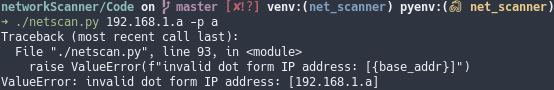
\includegraphics[width=\textwidth]{invalidipandport.png}
\caption{\textit{%
  screenshot of my program showing the output from an invalid ip and an invalid port number.
}}\label{invalidipandport}
\end{figure}

\subsection{Test Table}
\newcounter{row number}
\newcommand\rownumber{\stepcounter{row number}\arabic{row number}}
\begin{center}
  \begin{tabular}{r l l l r r}
    \toprule
    Test No. & Test Data & Expectation & Result & Fig & Success Criteria \\
    \midrule
    \rownumber{} & & usage message & Pass &\ref{noparametertest} &\ref{usage}  \\
    \rownumber{} & \verb| -h| & help message & Pass &\ref{hflagtest} &\ref{usage}  \\
    \rownumber{} & \verb|--help| & help message & Pass &\ref{helpflagtest} &\ref{usage}  \\
    \rownumber{} & \verb| -sL| & print addresses & Pass &\ref{cidrtest} &\ref{cidr}  \\
    \rownumber{} & \verb| -sn| & ping scan & Pass &\ref{lanscantest} &\ref{ping}  \\
    \rownumber{} & \verb| -Pn| & assume host up& Pass &\ref{nocheckoutput} &\ref{nocheck}  \\
    \rownumber{} & \verb$ -sS|sT$ & TCP port open& Pass &\ref{tcpopenoutput} &\ref{tcpopen}  \\
    \rownumber{} & \verb$ -sS|sT$ & TCP port closed& Pass &\ref{tcpclosedoutput} &\ref{tcpclosed}  \\
    \rownumber{} & \verb| -sS| & TCP port filtered& Pass &\ref{tcpfilteredoutput} &\ref{tcpfiltered}  \\
    \rownumber{} & \verb| -sU| & UDP port open& Pass &\ref{udpopenoutput} &\ref{udpopen}  \\
    \rownumber{} & \verb| -sU| & UDP port closed& Pass &\ref{udpclosedoutput} &\ref{udpclosed}  \\
    \rownumber{} & \verb| -sU| & UDP port filtered& Pass &\ref{udpfilteredoutput} &\ref{udpfiltered}  \\
    \rownumber{} & \verb| -sV| & OS detection & Partial &\ref{sshversiondetect} &\ref{osdetect}  \\
    \rownumber{} & \verb| -sV| & service detection & Pass &\ref{sshversiondetect} &\ref{servicedetect}  \\
    \rownumber{} & \verb| -sV| & version detection & Pass &\ref{sshversiondetect} &\ref{versiondetect}  \\
    \rownumber{} & & invalid IP & Pass &\ref{invalidip} & \\
    \rownumber{} & & invalid subnet & Pass &\ref{invalidnetworkbits} & \\
    \rownumber{} & & invalid port \& IP & Pass &\ref{invalidportnum} & \\
    \bottomrule
  \end{tabular}
\end{center}

\section{Evaluation}

\subsection{Reflection on final outcome}

Overall, I am very happy with how my program has turned out. At the beginning of this
project, I did not believe I could do anywhere near as much as I have done.
My rationale for choosing this project was to learn more about low level networking,
and networking in general, because these were areas where I felt my knowledge was deficient.
I greatly enjoyed learning about various aspects of networking structure and protocols.
For instance, I found it fascinating to discover that the order that bytes are packed into the packet matters
enormously, and to learn how users are automatically assigned an IP address on joining a network.

There were many areas where I encountered difficulty while developing this program.
The first problem was understanding what a packet is, and how I send one that I have made myself
using Python. There seemed to be very little in the way of documentation, so I ended up reading
many peoples' answers to questions on the Stack Overflow website, where they had encountered similar problems.
Once I discovered that I could simply open a socket in raw mode and use the \verb|socket.sendto|
method to send any arbitrary bytes to an address and Python would handle the IP header,
it became easier to make progress. The next major problem was getting the
checksum correct for \gls{tcp} packets, because they use a pseudo-header, which
is sort of a header made from fields in the \gls{ip} header that are not
in the \gls{tcp} header. They are used to calculate the checksum for the \gls{tcp}
header. Figuring out how to pack these properly, and in what endianness, turned out to be
one of the biggest difficulties in getting \gls{tcp} SYN scanning working.
I had a completely different problem when it came to implementing \gls{udp}
scanning. This is because when a \gls{udp} packet arrives and is destined for a closed port,
an \gls{icmp} destination unreachable message is sent back, and on Linux systems these are time-limited
to a maximum of one per second. 
Thus, I had to come up with a strategy that could deal with problem.
In the end, I added a maximum wait time for each packet sent, and instructed the program to listen
for that length of time to determine if an \gls{icmp} destination unreachable message was received.
Implementing version scanning came with its own difficulties.
Parsing the file which defines the probes and all the directives which are needed to interpret the service's
response was challenging, as was matching the returned data using a regular expression that was parsed from a file.

\subsection{Evaluation against objectives, end user feedback}
When I set out on this project I intended to make a program which was able to scan other
computers on a network from a \gls{bbox} perspective in a way similar to nmap.
Before commencing, I set out 14 pre-specified criteria against which the performance of my program
could be measured. As has been demonstrated above, the program fully meets 13 of the 14 criteria,
and partially meets the remaining criterion.
I believe therefore that my program has substantially met all the objectives set out
at the beginning.

\subsection{Potential improvements}
I believe that I could improve my program if it were to have a dedicated option for operating
system detection. 
It is clear that as a single individual, it would not be feasible for me to collect the required
number of operating system signatures myself. Therefore, in order to implement this feature,
I would need use another of the files from nmap: nmao-os-db, which contains
a database of \gls{tcp}/\gls{ip} stack fingerprints that show how the \gls{tcp} and \gls{ip}
protocols are implemented in virtually all currently-used operating systems, as well as in different
versions of Linux and different service packs and versions of Windows.

\clearpage
\appendix

\section{Technical Solution}\label{code}
\lstset{language=Python}
\subsection{icmp\_ping}\label{app:icmpping}
\lstinputlisting[caption=\textit{A prototype program for sending ICMP ECHO REQEST packets},label=icmpechosend]{../../Code/icmp_ping/icmp_echo_send.py}
\lstinputlisting[caption=\textit{A prototype program for receiving ICMP ECHO REQEST packets},label=icmpechorecv]{../../Code/icmp_ping/icmp_echo_recv.py}

\subsection{ping\_scanner}\label{app:pingscanner}
\lstinputlisting[caption=\textit{A prototype program for performing `ping' scans},label=pingscanner]{../../Code/ping_scanner/ping_scan.py}

\subsection{subnet\_to\_addresses}\label{app:subnettoaddresses}
\lstinputlisting[caption=\textit{A program which translates a CIDR specified subnet into a list of addresses and prints them out in sorted order},label=subnettoaddresses]{../../Code/subnet_to_address.py}

\subsection{tcp\_scan}\label{app:tcpscan}
\subsubsection{connect\_scan}\label{app:connectscan}
\lstinputlisting[caption=\textit{prototype TCP connect scanner only attempting to detect the state of port 22},label=connectsshattempt]{../../Code/tcp_scan/connect_scan/ssh_attempt.py}
\lstinputlisting[caption=\textit{A program that performs TCP connect scanning}, label=connectscanportlist]{../../Code/tcp_scan/connect_scan/scan_port_list.py}

\subsubsection{syn\_scan}\label{app:synscan}
\lstinputlisting[caption=\textit{A prototype program that tries to detect the state of port 22 via TCP SYN scanning (aka half open scanning)},label=synsshattempt]{../../Code/tcp_scan/syn_scan/ssh_attempt.py}
\lstinputlisting[caption=\textit{A program that performs TCP SYN scanning (aka half open scanning)},label=synscanportlist]{../../Code/tcp_scan/syn_scan/scan_port_list.py}

\subsection{udp\_scan}\label{app:udpscan}
\lstinputlisting[caption=\textit{A prototype program to detect whether UDP port 53 is open on a target machine}, label=dnsattempt]{../../Code/udp_scan/dns_attempt.py}
\lstinputlisting[caption=\textit{A program for performing scans on UDP ports.},label=udpscanportlist]{../../Code/udp_scan/scan_port_list.py}
\lstinputlisting[caption=\textit{A program I made to open a port via UDP for testing my UDP scanner.},label=openxport]{../../Code/udp_scan/open_X_port_to_UDP.py}

\subsection{version\_detection}\label{app:versiondetection}
\lstinputlisting[caption=\textit{A program which does version detection on services.},label=versiondetection]{../../Code/version_detection/version_detection.py}

\subsection{modules}\label{app:modules}
\lstinputlisting[caption=\textit{A Python module I wrote for parsing and holding the version detection probes from the nmap\_service\_probes file.},label=directives]{../../Code/modules/directives.py}
\lstinputlisting[caption=\textit{A Python module I made to dissect and hold protocol headers.},label=headers]{../../Code/modules/headers.py}
\lstinputlisting[caption=\textit{A Python module I wrote to contain lots of useful functions which I found I was declaring in multiple places and makign changes so I decided to keep an up to date central one.},label=iputils]{../../Code/modules/ip_utils.py}
\lstinputlisting[caption=\textit{A Python module I made to hold all of the listeners I had made for each of the different scanning types.},label=listeners]{../../Code/modules/listeners.py}
\lstinputlisting[caption=\textit{A Python module I made to hold all of the scanners I had made for each of the different scanning types.},label=scanners]{../../Code/modules/scanners.py}

\subsection{examples}\label{app:examples}
\lstinputlisting[caption=\textit{A program I wrote to run all of the example scripts I made from one main script to solve the issue of the PATH being used for determining import when I could use Pythons built in module structure instead.},label=runexamples]{../../Code/run_examples.py}

\subsection{netscan}\label{app:netscan}
\lstinputlisting[caption=\textit{The program which provides the command line user interface for my projects functionality.},label=netscan]{../../Code/netscan.py}

\subsection{tests}\label{app:tests}
\lstinputlisting[caption=\textit{Unit tests I wrote for the ip\_utils module.},label=testiputils]{../../Code/tests/test_ip_utils.py}
\lstinputlisting[caption=\textit{Unit tests I wrote for the directives module.},label=testdirectives]{../../Code/tests/test_directives.py}

\clearpage
\bibliographystyle{unsrt}
\nocite{*}
\bibliography{bibliography}


\clearpage
\printnoidxglossaries{}

\end{document}
